\documentclass[a4paper,11pt]{article}
\makeatletter
\def\input@path{{HwPolNotesNew/notes/}}
\makeatother
\usepackage{jheppub} % for details on the use of the package, please see the JINST-author-manual
\usepackage{lineno}
\usepackage{feynmp-auto}
\usepackage{subcaption}
\usepackage[section]{placeins}
\usepackage{flafter}
\usepackage{mathabx}
\usepackage{nicematrix}
\usepackage{fancyvrb}
\usepackage{snapshot}
\usepackage{slashed}
\VerbatimFootnotes
%\linenumbers
\newcommand{\beq}      {\begin{equation}}
\newcommand{\eeq}      {\end{equation}}
\newcommand{\beqn}     {\begin{eqnarray}}
\newcommand{\eeqn}     {\end{eqnarray}}
\newcommand{\slsh}     {\slashed}
\newcommand{\myfrac}[2]{\mbox{\small$\frac{#1}{#2}$}}
\newcommand{\half}     {\myfrac{1}{2}}
\newcommand{\ldot}[2]  {\:{#1}\!\cdot\!{#2}\:}
\newcommand{\Herwig}{\textsc{Herwig}}
\newcommand{\HerwigSeven}{\Herwig~7}
\newcommand{\Herwigpp}{\textsc{Herwig++}}
\newcommand{\POLDIS}{\textsc{POLDIS}}
\newcommand{\safegraphic}[2]{%
  \IfFileExists{#2}{%
    \includegraphics[width=#1]{#2}%
  }{%
    \fbox{\parbox[c][0.18\textheight][c]{#1}{\centering\footnotesize Diagram placeholder}}%
  }%
}

 
\title{\boldmath Polarized Deep-Inelastic Scattering with Spin Correlations in Herwig 7}

\author[1]{M.R.~Masouminia,}
\author[2]{A.~Papaefstathiou,}
\author[1]{P.~Richardson}
%
\affiliation[1]{Institute for Particle Physics Phenomenology, Durham University, Durham, UK}
\affiliation[2]{Department of Physics, Kennesaw State University, 830 Polytechnic Lane, Marietta, GA 30060, USA}


\emailAdd{mohammad.r.masouminia@durham.ac.uk}
\emailAdd{apapaefs@kennesaw.edu}
\emailAdd{peter.richardson@durham.ac.uk}

\abstract{Polarized deep-inelastic scattering (DIS) provides a direct probe of the spin structure of the nucleon and is a central element of the physics programme at the upcoming Electron--Ion Collider. We present an implementation of polarized DIS at next-to-leading order in \HerwigSeven\ using the POWHEG matching scheme, together with a consistent treatment of spin correlations for the realized real-emission configuration in NLO-matched events. The full spin-density matrix of the final state is propagated from the hard scattering to the parton shower without changing the matched hard-event normalization or the POWHEG emission choice. The integrated cross section is validated against fixed-order calculations, while differential hardest-emission proxy comparisons and exploratory shower-level observables are used to illustrate the impact of the new spin information at EIC energies.}




\begin{document}
\begin{flushright}
\footnotesize

IPPP-26-XX\\
MCNET-26-XX

\end{flushright}


\maketitle
\flushbottom

\section{Introduction}\label{sec:intro}

Polarized deep-inelastic scattering (DIS) provides one of the most direct probes of the spin structure of hadrons. The future Electron--Ion Collider (EIC) will combine polarized lepton and hadron beams with a broad kinematic reach and high luminosity, making it possible to study helicity-dependent partonic dynamics in unprecedented detail. In particular, fully differential measurements will provide new constraints on polarized parton distributions~\cite{Accardi:2012qut,AbdulKhalek:2021gbh}. To fully exploit such measurements, theoretical predictions must go beyond inclusive cross sections and provide a differential description that retains the correlations between kinematics, flavour, and spin in the hadronic final state.

The theoretical description of DIS has a long history. Building on the parton model and the QCD evolution equations~\cite{Altarelli:1977zs}, complete next-to-leading-order calculations for unpolarized DIS were already available by the late 1970s~\cite{Bardeen:1978yd}. Over the following decades this programme was extended to NNLO with the computation of the exact three-loop splitting functions~\cite{Moch:2004pa,Vogt:2004mw}, establishing DIS as one of the primary benchmark processes for precision PDF determinations. The polarized programme followed a parallel development, though with a significant time lag: NLO helicity-dependent radiative corrections and splitting functions were worked out in the mid-1990s~\cite{Mertig:1995ny,Vogelsang:1996im}, while the NNLO polarized ingredients, including the three-loop helicity-dependent splitting functions and the full set of inclusive polarized DIS structure functions, have only recently become available~\cite{Moch:2014sna,Borsa:2022nnlo}.

The emphasis of phenomenology has meanwhile shifted from inclusive calculations to fully differential event generation. This development led first to the general MC@NLO and POWHEG matching frameworks~\cite{Frixione:2002ik,Nason:2004rx,Frixione:2007vw}, and subsequently to DIS-specific NLO+PS implementations in \Herwig~\cite{DErrico:2011wfa}, in the POWHEG BOX for polarized DIS~\cite{Borsa:2024ps}, and, more recently, in dedicated POWHEG generators for lepton--hadron scattering with mass effects~\cite{Buonocore:2024dis}.

Within this broader programme, general-purpose Monte Carlo event generators provide the framework in which perturbative calculations can be combined with parton showers, hadronization, and decays to produce realistic event simulations. Among these, \Herwig\ combines perturbative hard-scattering calculations, parton showers, hadronization, and particle decays within a unified simulation framework~\cite{Bahr:2008pv,Gieseke:2011na,Arnold:2012fq,Bellm:2013hwb,Bellm:2015jjp,Bellm:2017bvx,Bellm:2019zci,Bewick:2023tfi,Bellm:2025pcw}, and already incorporates matching to higher-order corrections as well as a dedicated spin-correlation algorithm for propagating polarization information through showering and decays~\cite{Richardson:2018pvo}. An NLO-matched treatment of unpolarized DIS was implemented in an earlier version of the code~\cite{DErrico:2011wfa} via the POWHEG method. However, within \Herwig\ a corresponding polarized implementation, together with a mechanism for propagating the spin information of the realized real-emission configuration to the shower, has not previously been available.

In this paper we address both of these requirements. We present the implementation of polarized DIS in \Herwig\ at NLO accuracy via the POWHEG method, including the real-emission, virtual, and collinear-subtraction contributions required for matched event generation. This provides, within a general-purpose event generator, a spin-dependent description of the hard scattering itself, rather than relying only on the spin correlations generated by the shower alone. We note that this infrastructure establishes the ingredients needed for treating polarized hard scattering in \Herwig\ beyond the specific case of DIS considered here; extensions to other processes will be pursued in future work.

The second contribution concerns the propagation of spin information from the hard event to the parton shower. Once the hardest POWHEG emission has been generated, the accepted configuration is a specific real-emission state whose final-state particles carry correlated spin information. To preserve these correlations in the showered event, the parton shower must be initialized with the full spin-density information of the accepted real-emission state. We achieve this by constructing the spin-density matrix from the exact real-emission helicity amplitudes, and using it to initialize the shower, without modifying the accepted hard-event normalization or hardest-emission choice.

The remainder of this paper is organized as follows. In Section~\ref{sec:formalism} we review the spin-density-matrix formalism for polarized hadrons and the corresponding modifications to the parton shower. Section~\ref{sec:polarizeddis} presents the polarized DIS implementation, including the real and virtual contributions and their fixed-order validation, as well as the real-emission spin-correlation framework for the shower and the jet- and particle-level observables designed to isolate the phenomenological impact of the new spin information at EIC energies. We provide our conclusions and outlook in Section~\ref{sec:conclusions}.

\section{Formalism and Definitions}\label{sec:formalism}
\subsection{Polarized Hadrons}


For unpolarized hadrons, the relevant non-perturbative input is the parton distribution function $f_i(x,Q^2)$, giving the probability of finding a parton of type $i$ with momentum fraction $x$ at factorization scale $Q^2$.
Following the notation of Ref.\,\cite{Barone:2001sp}, for longitudinally polarized hadrons
we define the parton distributions $f_{i\pm}(x,Q^2)$ giving the probability of finding a parton of type $i$ with helicity $\pm$.
A difference parton distribution function $\Delta f_i(x,Q^2)$ is then introduced such that
\begin{subequations}
\begin{eqnarray}
  f_i(x,Q^2)        &=& f_{i+}(x,Q^2) + f_{i-}(x,Q^2),\\
  \Delta f_i(x,Q^2) &=& f_{i+}(x,Q^2) - f_{i-}(x,Q^2).
\end{eqnarray}
\end{subequations}
For transversely polarized hadrons, an additional distribution $\Delta_T f_i(x,Q^2)$ is required. It measures the difference between the probabilities of finding a parton with polarization parallel and antiparallel to that of the hadron; see Section 1 of Ref.\,\cite{Barone:2001sp} for details.

In terms of these distributions and the components of the hadron polarization vector in the $x,y,z$ directions,\footnote{Assuming the hadron is moving in the $z$ direction.} $P_{x,y,z}$,
we can define a spin density matrix\footnote{This is Eq.\ 4.3.7 of Ref.\,\cite{Barone:2001sp}, apart from a sign convention arising from our choice to order helicity states as $(-,+)$ rather than $(+,-)$.}
\begin{equation}
  H_{i\tau\tau'}(x,Q^2) = \frac12 \left( \begin{array}{cc} 1-\lambda(x,Q^2) & s_x(x,Q^2)+is_y(x,Q^2) \\ s_x(x,Q^2)-is_y(x,Q^2) & 1 + \lambda(x,Q^2) \end{array}\right),
\end{equation}
where
\begin{subequations}
  \begin{eqnarray}
    \lambda(x,Q^2) f_i(x,Q^2) &=& P_z \Delta f_i(x,Q^2), \\
    s_{x,y}(x,Q^2) f_i(x,Q^2) &=& P_{x,y} \Delta_T f_i(x,Q^2).
\end{eqnarray}
\end{subequations}

Considering a process with one incoming hadron, as in DIS, in which a parton of type $i$ initiates the process and $n$ particles are produced,
the differential cross section is given by
\begin{equation}
  \mathrm{d}\sigma_n = C \frac{(2\pi)^4}{2\hat{s}}\, \mathrm{d}x\, \mathrm{d}\Phi_n\, f_i(x,Q^2)\, H_{i\tau\tau'}(x,Q^2)\, \mathcal{M}_\tau\mathcal{M}^*_{\tau'}\;,\label{eqn:dsigma}
\end{equation}
where $\mathrm{d}\Phi_n$ is the differential phase space for the production of $n$ particles,
$C$ is the appropriate factor for summing over the colours and spins of the outgoing particles and averaging over those of the incoming particles, with the
exception of the spin of $i$. The matrix element for the process is $\mathcal{M}$, where the helicity indices of
all particles except $i$ have been suppressed for clarity. For unpolarized hadrons $H_{i\tau\tau'}(x,Q^2)\to 1/s_i\,\delta_{\tau\tau'}$, where $s_i$ is the number of spin states for parton $i$, and
Eq.~\eqref{eqn:dsigma} reduces to the standard cross section formula.

The spin-density matrix $H_{i\tau\tau'}$ defined here enters directly in the parton shower evolution discussed in the next subsection, and its generalization to the NLO real-emission state is the subject of Section~\ref{sec:polarizeddis}.

\subsection{Parton Shower Evolution}

The differential cross section including a single initial-state emission takes the form
\begin{equation}
 \mathrm{d}\sigma_{n+1} = \frac{\mathrm{d}z}z \frac{\mathrm{d}Q^2}{Q^2} \frac{\mathrm{d}\phi}{2\pi}\frac{\alpha_s}{2\pi}\,
 C \frac{(2\pi)^4}{2\hat{s}}\, \mathrm{d}x\, \mathrm{d}\Phi_n\,
 f_i\left(x/z,Q^2\right)\, H_{i\lambda_0\lambda'_0}\left(x/z,Q^2\right)\,
 F_{\lambda_0\lambda_1\lambda_2} F^*_{\lambda'_0\lambda'_1\lambda_2}\,
 \mathcal{M}_{\lambda_1}\mathcal{M}^*_{\lambda_1'}\;,
\end{equation}
where $F_{\lambda_0\lambda_1\lambda_2}$ are the helicity amplitudes for the branching, defined in Ref.\,\cite{Richardson:2018pvo} such that
\begin{equation}
  P_{i\to jk}(z) = \frac12\sum_{\lambda_0,\lambda_1,\lambda_2}  F_{\lambda_0\lambda_1\lambda_2} F^*_{\lambda_0\lambda_1\lambda_2}\;,
\end{equation}
where $P_{i\to jk}(z)$ is the standard spin-averaged splitting function for the branching $i\to jk$.

The differential branching probability is then
\begin{equation}
  \mathrm{d}\mathcal{P} = \frac{\mathrm{d}z}z \frac{\mathrm{d}Q^2}{Q^2} \frac{\mathrm{d}\phi}{2\pi}\frac{\alpha_s}{2\pi}\,
  \frac{f_i\left(x/z,Q^2\right) }{ f_j(x,Q^2) }
  \frac{H_{i\lambda_0\lambda'_0}\left(x/z,Q^2\right) F_{\lambda_0\lambda_1\lambda_2} F^*_{\lambda'_0\lambda'_1\lambda_2} \mathcal{M}_{\lambda_1}\mathcal{M}^*_{\lambda_1'}}{H_{j\tau\tau'}(x,Q^2) \mathcal{M}_\tau\mathcal{M}^*_{\tau'}}\;.
\end{equation}
For unpolarized hadrons this reduces to
\begin{equation}
  \mathrm{d}\mathcal{P} = \frac{\mathrm{d}z}z \frac{\mathrm{d}Q^2}{Q^2} \frac{\mathrm{d}\phi}{2\pi}\frac{\alpha_s}{2\pi}\,
  \frac{f_i\left(x/z,Q^2\right) }{ f_j(x,Q^2) }
  F_{\lambda_0\lambda_1\lambda_2} F^*_{\lambda_0\lambda'_1\lambda_2} D_{\lambda_1\lambda_1'}\;,
\end{equation}
where the decay matrix is given by
\begin{equation}
  D_{\lambda\lambda'} = \frac{\mathcal{M}_{\lambda}\mathcal{M}^*_{\lambda'}}{\mathcal{M}_\tau\mathcal{M}^*_{\tau}}\;.
\end{equation}
If spin correlations between the emission and the hard process are neglected, $D_{\lambda\lambda'}\to \frac12\delta_{\lambda\lambda'}$,
and one recovers the standard result
\begin{equation} 
  \mathrm{d}\mathcal{P}_\mathrm{uncorrelated} = \frac{\mathrm{d}z}z \frac{\mathrm{d}Q^2}{Q^2} \frac{\alpha_s}{2\pi}\,
  \frac{f_i\left(x/z,Q^2\right) }{ f_j(x,Q^2) } P_{i\to jk}(z)\;.
\end{equation}
Rewriting the full branching probability in terms of $\mathrm{d}\mathcal{P}_\mathrm{uncorrelated}$,
\begin{equation}
  \mathrm{d}\mathcal{P} = \mathrm{d}\mathcal{P}_\mathrm{uncorrelated} W_\mathrm{correlated}\;,
\end{equation}
where
\begin{equation}
  W_\mathrm{correlated} =
  \frac{\mathrm{d}\phi}{2\pi}\frac1{2H_{j\tau\tau'}(x,Q^2) D_{\tau\tau'}}
  \frac{2H_{i\lambda_0\lambda'_0}\left(x/z,Q^2\right) F_{\lambda_0\lambda_1\lambda_2} F^*_{\lambda'_0\lambda'_1\lambda_2}D_{\lambda_1\lambda_1'}}{P_{i\to jk}(z)}\;,
\end{equation}
where each factor reduces to unity in the absence of beam polarization and spin correlations, respectively.
We can write the second ratio in the form
\begin{equation}
   \frac{2H_{i\lambda_0\lambda'_0}\left(x/z,Q^2\right) F_{\lambda_0\lambda_1\lambda_2} F^*_{\lambda'_0\lambda'_1\lambda_2}D_{\lambda_1\lambda_1'}}{P_{i\to jk}(z)} = 1 + A + B + C\,,\label{eqn:corr}
\end{equation}
where $A$ is azimuthally independent and contributes only for polarized hadrons; $B$ is azimuthally dependent and present even for unpolarized beams; and $C$ is azimuthally dependent but contributes only for polarized hadrons.
The values of $A$, $B$ and $C$ are given in Tables\,\ref{tab:branch1} and \ref{tab:branch2} where the condition that both $H_i$ and $D$ have unit trace
has been used to simplify the results.

The azimuthal dependence of $B$ and $C$ is proportional to $e^{\pm 2 i\phi}$ and therefore averages to zero upon integration over the full azimuth.
In the present study we restrict attention to longitudinal beam polarization, for which $H_{i+-}=H_{i-+}=0$ for all parton species; in particular $H_{g\pm\mp}=0$ for spin-$\frac12$ hadrons. The off-diagonal terms therefore do not contribute in the present context. Extending the framework to transverse polarization would require transversity PDFs in the quark channels together with a dedicated rederivation of the corresponding hard and collinear spin structures in a transverse-spin basis; for a spin-$\frac12$ hadron there is no leading-twist gluon transversity. We therefore retain the off-diagonal terms only as future-facing notation, e.g.\ for transversely polarized hadrons or polarized resolved-photon processes.
\begin{table}
  \begin{center}
    \begin{tabular}{|c|c|}
      \hline
      Branching & A \\
      \hline
      $q\to qg$ & $\lambda(x,Q^2) \left(D_{++}-D_{--}\right)+\frac{4 z}{1+z^2} \left(H_{i-+}(x/z,Q^2)D_{-+} +H_{i+-}(x/z,Q^2)D_{+-} \right)$ \\
      \hline
      $q\to gq$ & $\lambda(x,Q^2) \frac{  (2-z) z}{1+(1-z)^2} \left(D_{++}-D_{--}\right)$ \\
      \hline
      $g\to gg$ & $\lambda(x,Q^2) \frac{z (2-z -2z(1-z))}{(1-(1-z) z)^2} \left(D_{++}-D_{--}\right)$ \\
      & $+\frac{2 z^2}{(1-(1-z)z)^2}\left(D_{-+} H_{i-+}(x/z,Q^2)+D_{+-}H_{i+-}(x/z,Q^2)\right)$\\
      \hline
      $g\to q\bar{q}$ & $-\lambda(x,Q^2) \frac{1-2 z}{1-2 (1-z) z}\left(D_{++}-D_{--}\right)$ \\
      \hline
  \end{tabular}
    \caption{Azimuthal-independent spin weights for the different possible QCD branchings.}
    \label{tab:branch1}
  \end{center}
\end{table}

\begin{table}
  \begin{center}
    \begin{tabular}{|c|c|c|}
      \hline
      Branching & B & C \\
      \hline
      $q\to qg$ & 0 & 0 \\
      \hline
      $q\to gq$ & $-\frac{2 (1-z)}{1+(1-z)^2} \left(e^{2 i \phi } D_{-+}+e^{-2 i \phi } D_{+-}\right)$& 0 \\
      \hline
      $g\to gg$ & $-\frac{(1-z)^2}{(1-(1-z) z)^2} \left(e^{2 i \phi } D_{-+}+e^{-2 i \phi } D_{+-}\right)$ & $-\frac{z^2 (1-z)^2 \left(e^{-2 i \phi } H_{i-+}(x/z,Q^2)+e^{2 i \phi }H_{i+-}(x/z,Q^2)\right)}{(1-(1-z) z)^2}$\\
      \hline
      $g\to q\bar{q}$ & 0 &  $\frac{2 (1-z) z \left(e^{-2 i \phi } H_{i-+}(x/z,Q^2)+e^{2 i \phi } H_{i+-}(x/z,Q^2)\right)}{1-2 (1-z) z}$\\
      \hline
  \end{tabular}
    \caption{Azimuthal-dependent spin weights for the different possible QCD branchings.}
    \label{tab:branch2}
  \end{center}
\end{table}

We can therefore generate the branching probability, averaged over $\phi$ as before, with the additional weight
\begin{equation}
  W_\mathrm{uncorrelated} = \frac{1+A}{2H_{j\tau\tau'}(x,Q^2) D_{\tau\tau'}}\;,
\end{equation}
which can be included in the normal weight for the PDF term. The azimuthal angle can then be generated using the full distribution in Eq.~\eqref{eqn:corr} rather than
using only the $1+B$ distribution that applies in the unpolarized case. The decay matrix $D$ is then updated to include the branching and used to initialize the next emission. Once the backward evolution terminates, the spin-averaged density matrix $\rho$ is replaced by the full hadronic spin-density matrix $H_{i\lambda\lambda'}$. The chain is then traversed in the forward direction to initialize the final-state showers of the radiated partons.

The formalism developed in this section applies to shower emissions that evolve from a Born-level hard process. Its extension to the case in which the shower is instead seeded by a realized NLO real-emission configuration is described in Section~\ref{sec:polarizeddis}.

\section{Polarized Deep-Inelastic Scattering}\label{sec:polarizeddis}

In this section we present the polarized DIS implementation developed in
\Herwig. We first derive the real-emission contributions and then discuss the
virtual terms and collinear remainders needed for a complete NLO calculation. We
next validate these ingredients in fixed-order-like comparisons before turning
to the new shower-level treatment, in which the spin information of the
realized real-emission state is propagated through the parton shower and tested
with dedicated spin-sensitive observables.

For convenience, Table~\ref{tab:dis-notation-summary} summarizes the main kinematic variables and channel-dependent labels used in the real-emission derivation.

\begin{table}[t]
  \centering
  \footnotesize
  \setlength{\tabcolsep}{4pt}
  \begin{tabular}{|p{0.11\textwidth}|p{0.28\textwidth}|p{0.37\textwidth}|}
    \hline
    Symbol & Channel assignment & Meaning \\
    \hline
    $x_B$ & Same in QCDC and BGF & Bjorken scaling variable of the underlying Born DIS configuration. \\
    \hline
    $x_p$ & QCDC: incoming quark; BGF: incoming gluon & Real-emission momentum-fraction variable, so that the incoming parton in the kernel carries $x=x_B/x_p$. \\
    \hline
    $z_p$ & In both channels: outgoing-quark fraction & Phase-space variable used to parameterize the real-emission region and its collinear limits. \\
    \hline
    $x_1,x_2,x_3$ & QCDC: incoming quark, outgoing quark, gluon; BGF: incoming gluon, outgoing quark, outgoing antiquark & Channel-dependent Breit-frame momentum fractions entering the CALKUL factorization. \\
    \hline
    $r_i,\bar r_i$ & Definitions differ between QCDC and BGF & Auxiliary massless mapped momenta used to factorize the real matrix element onto Born-like DIS kinematics. \\
    \hline
  \end{tabular}
  \caption{Summary of the channel-dependent notation used in Section~\ref{sec:realconts}. The labels $x_1,x_2,x_3$ and the mapped momenta $r_i,\bar r_i$ refer to different external legs in QCDC and BGF.}
  \label{tab:dis-notation-summary}
\end{table}

\subsection{Real emission contributions}
\label{sec:realconts}

\subsubsection{QCD Compton scattering}

\begin{figure}[htbp]
\safegraphic{0.47\linewidth}{figures/QCDC1.png}
\safegraphic{0.47\linewidth}{figures/QCDC2.png}

\par\bigskip
    \caption{The QCD Compton process.}
    \label{fig:realemission}
\end{figure}

With reference to the diagrams in Fig.~\ref{fig:realemission}, the matrix element for the process $eq \to eqg$, where the outgoing quark has helicity $\lambda$ and the emitted gluon has helicity $\rho$, is given by
\begin{equation}
  \mathcal{M} _3(\lambda,\rho) = ig_s\bar{u}_\lambda(p_2)
  \left[\slsh\epsilon_\rho(p_3)\frac{-(\slsh p_2+\slsh p_3)}{2\ldot{p_2}{p_3}}
        \omega^\mu+\omega^\mu\frac{-(\slsh p_1-\slsh p_3)}{-2\ldot{p_1}{p_3}}
        \slsh\epsilon_\rho(p_3)\right]u_\lambda(p_1)J_\mu(q) T^a_{ij}\;,
\end{equation}
where the momentum of the incoming (outgoing) quark is $p_1$ ($p_2$), and that of the gluon is $p_3$. The four-vector $\omega^\mu = (V_q + A_q \gamma^5)\gamma^\mu$ represents a general boson--quark coupling, and the $T^a_{ij}$ are the SU(3) generator matrix elements. All partons are taken to be massless, so that quark chirality -- and hence helicity -- is conserved. We adopt the CALKUL gluon-polarization tensor~\cite{DeCausmaecker:1981jtq}, in which the two diagrams contribute to physically distinct helicity configurations, and all interference is absorbed into the definition of $\epsilon_\rho$:
\begin{align}
  \slsh\epsilon_\rho(k, p_1, p_2) &= N\left(
    \half(1+\rho\gamma^5)\slsh k\slsh p_2\slsh p_1 -
    \slsh p_2\slsh p_1\slsh k\half(1+\rho\gamma^5) \right), \\
  N(k,p_1,p_2) &= \left[ 4 \ldot{p_1}{k} \ldot{p_2}{k} \ldot{p_1}{p_2}
    \right]^{-\half}.
\end{align}
After some Dirac algebra, using the massless on-shell condition, we obtain
\begin{align}
  \mathcal{M}_3^+\equiv\mathcal{M}_3(\lambda,\phantom{-}\lambda) &=
    -ig_sN\bar{u}_\lambda(p_2)\omega^\mu(\slsh p_1-\slsh p_3)\slsh p_2
    u_\lambda(p_1)J_\mu(q)T^a_{ij}\;, \\
  \mathcal{M}_3^-\equiv\mathcal{M}_3(\lambda,-\lambda) &=
    -ig_sN\bar{u}_\lambda(p_2)\slsh p_1(\slsh p_2+\slsh p_3)\omega^\mu
    u_\lambda(p_1)J_\mu(q)T^a_{ij}\;.
\end{align}
We first define the momentum fractions
\begin{align}\label{eq:xi}
x_i \equiv \frac{ 2 \ldot{p_i}{q} } {\ldot{q}{q}}\;,
\end{align}
with $x_1 \leq -1$ and $x_2 \leq 1$, where the equalities are reached at the Born level; in the real-emission region one has $x_1<-1$ and $x_2<1$.
In terms of these, we introduce the auxiliary vectors
\begin{align}
  r_1       &\equiv          - p_1/x_1,\\
  \bar{r}_2 &\equiv \phantom{-}r_1+q=p_2+p_3-p_1-p_1/x_1,\\
  r_2       &\equiv \phantom{-}p_2/x_2,\\
  \bar{r}_1 &\equiv \phantom{-}r_2-q=p_1-p_3-p_2+p_2/x_2.
\end{align}
The vectors $r_1$ and $\bar{r}_2$ coincide with the incoming and outgoing quark momenta at leading order (where $x_1=-1$ and $p_3=0$) for the same values of $y_B$ and $Q^2$. By contrast, $r_2$ remains collinear with the physical outgoing quark momentum $p_2$, while $\bar{r}_1$ carries the compensating transverse recoil relative to the current direction.

These vectors allow the matrix elements to be cast in a factorized form. Momentum conservation at the boson--quark vertex gives $p_1+q=p_2+p_3$. Using these relations together with the identities
\begin{align}
      u(\alpha p) &\cong \sqrt\alpha\,u(p)\qquad (\alpha>0), \\
      (\slsh p_1 - \slsh p_3) \slsh p_2 &= \left(\slsh p_1 - \slsh p_3 - \slsh p_2 + \frac{\slsh p_2 }{x_2} \right) \slsh p_2\\
      &= \left(-\slsh q + \frac{\slsh p_2}{x_2}\right)\slsh p_2
      = \slashed{\bar{r}_1} \slsh p_2 = u_\lambda(\bar{r}_1)\, \bar{u}_\lambda(\bar{r}_1)\, \slsh p_2\;,\\
      \slsh p_1 (\slsh p_2 + \slsh p_3) &= \slsh p_1 \left( \slsh p_2 + \slsh p_3 - \slsh p_1 - \frac{\slsh p_1 }{ x_1 } \right) \\
      &= \slsh p_1 \left(\slsh q - \frac{\slsh p_1}{x_1}\right) =\slsh p_1 \slashed{\bar{r}_2} \\
      &= \slsh p_1\, u_\lambda(\bar{r}_2)\, \bar{u}_\lambda(\bar{r}_2)\;,
\end{align}
where $\cong$ denotes equality up to an overall complex phase that cancels in $|\mathcal{M}|^2$. For the crossed initial-state factor with $x_1<0$, the spinor rescaling is understood through its crossed analytic continuation; we therefore write the modulus explicitly as $\sqrt{|x_1|}$ and absorb the associated phase into the coefficient $C^-$. The corresponding analytic-continuation phase then drops out of $|C^-|^2$. Inserting these into the matrix elements we obtain
\begin{align}
  \mathcal{M}_3^+ &\cong g_sN\sqrt{x_2}\;\bar{u}_\lambda(r_2)
    \omega^\mu u_\lambda(\bar{r}_1)\bar{u}_\lambda(\bar{r}_1)\slsh p_2
    u_\lambda(p_1)J_\mu(q)\,T^a_{ij} \\
  &\equiv C^+\widetilde{\mathcal{M}}_2(\bar{r}_1,r_2)\,T^a_{ij} ,\\
  C^+ &= g_sN\sqrt{x_2}\;\bar{u}_\lambda(\bar{r}_1)
    \slsh p_2u_\lambda(p_1)\;, \\
  \mathcal{M}_3^- &\cong C^-\widetilde{\mathcal{M}}_2(r_1,\bar{r}_2)\,T^a_{ij} ,\\
  C^- &= g_sN\sqrt{|x_1|}\,e^{i\varphi_1}\;\bar{u}_\lambda(p_2)
    \slsh p_1u_\lambda(\bar{r}_2)\;,
\end{align}
where $\widetilde{\mathcal{M}}_2(q_1,q_2)=\bar{u}_\lambda(q_2) \omega^\mu u_\lambda(q_1)
 J_\mu(q)$ is the colour-stripped Born matrix element for the current to scatter
 an incoming quark $q_1$ to an outgoing quark $q_2$, and $e^{i\varphi_1}$ denotes the crossing phase associated with $x_1<0$. The real-emission colour factor $T^a_{ij}$ is kept outside $\widetilde{\mathcal{M}}_2$ and yields the overall $C_F$ only after the colour trace in the squared matrix element. Finally, using the relation\footnote{See, e.g., ref.~\cite{DeCausmaecker:1981jtq}}
\begin{align}
u_\pm(p) \bar{u}_\pm(p) = \half (1 \pm \gamma^5)\,\slsh p\;,
\end{align}
we obtain the explicit expressions
\begin{align}
  |C^+|^2 &= \frac{8\pi\alpha_s}{(-1-x_1)(1-x_2)Q^2} x_2^2 ,\\
  |C^-|^2 &= \frac{8\pi\alpha_s}{(-1-x_1)(1-x_2)Q^2} x_1^2 .
\end{align}

In the Breit frame, defined by $q=(0;0,0,-Q)$ or equivalently $2x_B P+q=0$, the four-momenta of the leading-order partons and exchanged boson are:
\begin{align}
\tilde{p}_1 &= \frac{Q}2(1;0,0,1)\;;\\
\tilde{p}_2 &= \frac{Q}2(1;0,0,-1)\;;\\
q &= Q(0;0,0,-1)\;,
\end{align}
where the tilde denotes leading-order quantities. In this frame, the four-momenta of the real-emission process are:
\begin{align}
p_1 &= \frac{Q}2(-x_1;0,0,-x_1)\;;\\
p_2 &= \frac{Q}2(\sqrt{x^2_2+x_\perp^2};\phantom{-}x_\perp\cos\phi,
                                        \phantom{-}x_\perp\sin\phi,-x_2)\;;\\
p_3 &= \frac{Q}2(\sqrt{x^2_3+x_\perp^2};          -x_\perp\cos\phi,
                                                  -x_\perp\sin\phi,-x_3)\;,
\end{align}
where the $x_i$ have been defined in Eq.~\eqref{eq:xi}. Here $x_B=Q^2/(2P\cdot q)$ is the usual Bjorken scaling variable, and below we use $y_B=(P\cdot q)/(P\cdot q_1)$ for the DIS inelasticity. Imposing momentum conservation, $x_{3}=2+x_{1}-x_{2}$, the transverse component is
\begin{equation}
x_\perp^2 = \frac{(x_3^2-x_1^2-x_2^2)^2}{4x_1^2}-x^2_2\;.
\end{equation}


With these kinematics, the leading-order cross section takes the form\footnote{At Born level the exchanged electroweak boson is colour singlet, so the colour structure is just $\delta_{ij}$ and its sum/average reduces to unity; the colour dependence is therefore implicit in $\mathrm{d}\Gamma_2$ and does not appear as a separate factor multiplying $|\widetilde{\mathcal{M}}_2|^2$.}
\begin{align}
  \mathrm{d} \sigma_2 &= \frac{1}{64\pi}\;\frac{1}{s^2 x_B^2}f_q(x_B,Q^2)
    \mathrm{d} Q^2\, \mathrm{d} x_B\, \frac{\mathrm{d}\Phi}{2\pi}\; |\widetilde{\mathcal{M}}_2(\tilde{p}_1,\tilde{p}_2)|^2 \\
  &\equiv \mathrm{d} \Gamma_2 |\widetilde{\mathcal{M}}_2(\tilde{p}_1,\tilde{p}_2)|^2\;.
\end{align}
Here $\mathrm{d}\Gamma_2$ is a compact shorthand for the Born-level flux, PDF, and phase-space measure appearing in the first line, rather than a pure invariant phase-space element alone. We use uppercase $\Phi$ for Born or underlying-Born phase-space orientations and lowercase $\phi$ for the real-emission radiation azimuth. Here $\Phi$ denotes the azimuthal orientation of the Born DIS scattering plane in the Breit frame.
The real-emission cross section is
\begin{align}
  \mathrm{d}\sigma_3 &= \frac{C_F}{128(2\pi)^3}\;\frac{1}{s^2x_B^2}
    f_q(-x_B x_1,Q^2)
    \mathrm{d} Q^2\, \mathrm{d} x_B\,\frac{\mathrm{d}\Phi}{2\pi}\frac{\mathrm{d} x_1}{x_1^2}\mathrm{d}x_2\frac{\mathrm{d} \phi}{2\pi}\;
    Q^2 |\mathcal{M}_3|^2 \\
  &= \frac{C_F}{4(2\pi)^2}\mathrm{d}\Gamma_2
    \frac{-x_B x_1f_q(-x_B x_1,Q^2)}
         { x_B    f_q( x_B    ,Q^2)}
    \frac{\mathrm{d} x_1}{-x_1^3}\mathrm{d}x_2
    \frac{\mathrm{d}\phi}{2\pi}\;
    Q^2 |\mathcal{M}_3|^2 \\
  &= \frac{C_F\alpha_s}{2\pi}\mathrm{d}\Gamma_2
    \frac{-x_B x_1f_q(-x_B x_1,Q^2)}
         { x_B    f_q( x_B    ,Q^2)}
    \frac{\mathrm{d} x_1 \mathrm{d}x_2}{-x_1^3(-1-x_1)(1-x_2)}\;\frac{\mathrm{d}\phi}{2\pi}
\nonumber\\&
   \times \left[ x_1^2|\widetilde{\mathcal{M}}_2(r_1,\bar{r}_2)|^2 +
           x_2^2|\widetilde{\mathcal{M}}_2(\bar{r}_1,r_2)|^2 \right]\;,
\label{eq:QCDC1}
\end{align}
where we have performed the colour trace. We now introduce the phase-space variables $x_p \equiv -1/x_1$ and
\begin{equation}
z_p \equiv \frac{\ldot{p_2}{P}}{\ldot{q}{P}} = 1 + \frac{1-x_2}{x_1}\;,
\end{equation}
where $P$ is the incoming hadron momentum. In terms of these variables, the phase-space limits factorize:
\begin{eqnarray}
  x_B \;<& x_p &<\; 1\;, \\
        0 \;<& z_p &<\; 1\;.
\end{eqnarray}
Inverting these relations gives
\begin{align}
  x_1 &= -\frac{1}{x_p}\;, \\
  x_2 &= 1-\frac{1-z_p}{x_p}\;.
\end{align}
The third momentum fraction follows from momentum conservation as
\begin{equation}
  x_3 = 2+x_1-x_2 = 1-\frac{z_p}{x_p}\;.
\end{equation}
The Jacobian for the transformation is
\begin{equation}
  \left|\frac{\partial(x_1,x_2)}{\partial(x_p,z_p)}\right| = \frac{1}{x_p^3}\;,
\end{equation}
so that
\begin{equation}
  \frac{\mathrm{d} x_1 \mathrm{d}x_2}{-x_1^3(-1-x_1)(1-x_2)}
  = x_p^2\,\frac{\mathrm{d} x_p \mathrm{d}z_p}{(1-x_p)(1-z_p)}\;,
\end{equation}
because $-x_1^3=1/x_p^3$, $-1-x_1=(1-x_p)/x_p$, and $1-x_2=(1-z_p)/x_p$. Moreover,
\begin{equation}
  x_3^2-x_1^2-x_2^2 = -\,\frac{2(2x_pz_p-x_p-z_p+1)}{x_p^2}\;.
\end{equation}
The transverse momentum in units of $Q/2$ is
\begin{equation}
  x_\perp^2 = \frac{4(1-x_p)(1-z_p)z_p}{x_p}\;,
\end{equation}
and therefore
\begin{equation}
  x_p^2(x_2^2+x_\perp^2) = (2x_pz_p-x_p-z_p+1)^2\;.
\end{equation}
Substituting these relations into Eq.~\eqref{eq:QCDC1} yields the real-emission cross section:
\begin{align}
  \mathrm{d}\sigma_3 &= \frac{C_F\alpha_s}{2\pi}\frac{\mathrm{d}\phi}{2\pi}
    \frac{\frac{x_B}{x_p} f_q(x_B/x_p,Q^2)}
         { x_B    f_q( x_B    ,Q^2)}
    \frac{\mathrm{d} x_p \mathrm{d}z_p}{(1-x_p)(1-z_p)}\;
\nonumber\\&
   \times \mathrm{d} \Gamma_2 \left\{ |\widetilde{\mathcal{M}}_2(r_1,\bar{r}_2)|^2 +
        x_p^2 x_2^2 |\widetilde{\mathcal{M}}_2(\bar{r}_1,r_2)|^2 \right\}\;.
\label{eq:QCDC2}
\end{align}
Since $r_1 = -p_1/x_1$ and $\bar{r}_2 = r_1 + q$, the pair $(r_1,\bar{r}_2)$ defines a Born-like DIS configuration with the same $Q^2$, $y_B$, and azimuthal angle as the mapped leading-order point. The factor $\mathrm{d} \Gamma_2 |\widetilde{\mathcal{M}}_2(r_1,\bar{r}_2)|^2$ is therefore precisely the corresponding leading-order differential cross section, which we denote again by $\mathrm{d}\sigma_2$. Defining
\begin{align}\label{eq:R2}
R_2 \equiv \frac{x_2^2}{x^2_2+x^2_\perp} \frac{|\widetilde{\mathcal{M}}_2(\bar{r}_1,r_2)|^2}{|\widetilde{\mathcal{M}}_2(r_1,\bar{r}_2)|^2}\;,
\end{align}
so that
\begin{equation}
  x_2^2 |\widetilde{\mathcal{M}}_2(\bar{r}_1,r_2)|^2
  = (x_2^2+x_\perp^2) R_2 |\widetilde{\mathcal{M}}_2(r_1,\bar{r}_2)|^2\;,
\end{equation}
we can write
\begin{align}
  \mathrm{d}\sigma_3 &= \frac{C_F\alpha_s}{2\pi}\frac{\mathrm{d}\phi}{2\pi}
    \frac{\frac{x_B}{x_p} f_q(x_B/x_p,Q^2)}
         { x_B    f_q( x_B    ,Q^2)}
    \frac{\mathrm{d} x_p \mathrm{d}z_p}{(1-x_p)(1-z_p)} \left\{ 1 +
         x_p^2 (x_2^2 + x_\perp^2) R_2 \right\} \mathrm{d} \sigma_2\;,
\label{eq:QCDC3}
\end{align}
Specializing to $ep$ scattering, the four-momenta of the incoming and outgoing leptons in the Breit frame are, respectively,
\begin{align}
q_1 &= \frac{Q}2(\ell;\sqrt{\ell^2-1},0,-1)\;;\\
q_2 &= \frac{Q}2(\ell;\sqrt{\ell^2-1},0,1)\;.
\end{align}
where, equivalently at the parton level, $y_B=\ldot{p_1}{q}/\ldot{p_1}{q_1}$ gives $\ell = 2/y_B -1$, and $\ell Q/2$ is the energy of the incoming lepton in the Breit frame. Defining $\cos\theta_2 = x_2 / \sqrt{x_2^2 + x_\perp^2}$, we then obtain
\begin{align}\label{eq:R2expression}
R_2 = \frac{\cos^2\theta_2+\mathcal{A}\cos\theta_2\left(\ell-\sqrt{\ell^2-1}\sin\theta_2\cos\phi\right)+\left(\ell-\sqrt{\ell^2-1}\sin\theta_2\cos\phi\right)^2}{1+\mathcal{A}\ell+\ell^2},
\end{align}
The denominator is the Born DIS angular factor: the lowest-order
matrix element squared expressed in the same Breit-frame variables,
with the overall coupling normalization factored out. Here
$\mathcal{A}=0$ for pure photon exchange, while for charged-current
DIS one has $\mathcal{A}=2$ in the default $e^-q$ orientation, with
the sign flipping upon crossing either the lepton or quark
line. Unless stated otherwise, the neutral-current formulas displayed
in this subsection are written for the default $e^-q$ orientation;
crossed channels are obtained later through the explicit
$\eta_\ell,\eta_q$ substitutions. We define the couplings
\begin{align}
C_{V,i} &= \frac{1}{\sin\theta_W \cos\theta_W} \left(\frac{T_{3,i}}{2} - Q_i \sin^2 \theta_W\right)\;,\\
C_{A,i} &= \frac{1}{\sin\theta_W \cos\theta_W} \frac{T_{3,i}}{2}\;,
\end{align}
where $\theta_W$ is the Weinberg angle, $T_{3,i}$ and $Q_i$ are the
weak isospin and charge of the fermion, respectively. For the full
neutral-current case, including $\gamma/Z$ interference, we then have
\begin{align}\label{eq:Aunpol}
\mathcal{A} = \frac{4 r C_{A,\ell} C_{A,q} \left(Q_\ell Q_q+2rC_{V,\ell}C_{V,q} \right)}
{\left(Q_\ell^2Q_q^2+2Q_\ell Q_q rC_{V,\ell}C_{V,q}
+r^2\left(C^2_{V,\ell}+C^2_{A,\ell}\right)\left(C^2_{V,q   }+C^2_{A,q   }\right)\right)},
\end{align}
with $r=\frac{Q^2}{(Q^2+m^2_Z)}$, where $m_Z$ is the $Z$ boson mass. In the code the exact finite-width propagator factors
\begin{equation}
  \chi_{\gamma Z}(Q^2)=\frac{Q^2(Q^2+m_Z^2)}{(Q^2+m_Z^2)^2+m_Z^2\Gamma_Z^2}\,,
  \qquad
  \chi_{ZZ}(Q^2)=\frac{Q^4}{(Q^2+m_Z^2)^2+m_Z^2\Gamma_Z^2}
\end{equation}
are used instead. With the present conventions for $C_{V,i}$ and $C_{A,i}$, the exact-width result is obtained algebraically by replacing every interference-term factor $r$ by $\chi_{\gamma Z}(Q^2)$ and every pure-$Z$ factor $r^2$ by $\chi_{ZZ}(Q^2)$, without introducing any additional powers of $\sin\theta_W\cos\theta_W$.

\paragraph{Polarized case.}
Up to this point we have worked under the assumption of unpolarized incoming partons. The same procedure applies to definite-helicity incoming partons with polarizations $P_\ell, P_q=\pm 1$, yielding $\mathrm{d} \sigma_3^{P_\ell,P_q}$ with $\mathrm{d}\sigma_2^{P_\ell,P_q}$ appearing in Eq.~\eqref{eq:QCDC3}. The same functional form for $R_2$ arises as in Eq.~\eqref{eq:R2expression}. The relevant amplitudes have been calculated using the \texttt{FeynCalc} package~\cite{Mertig:1990an,Shtabovenko:2016sxi,Shtabovenko:2020gxv,Shtabovenko:2023idz} to yield, for the full neutral-current case,
\begin{align}\label{eq:APol}
\mathcal{A}^{NC}_{P_\ell,P_q} = \frac{ N_0 + P_\ell N_\ell + P_q N_q + P_\ell P_q N_{\ell q}} {D_0 + P_\ell D_\ell + P_q D_q + P_\ell P_q D_{\ell q} }\;,
\end{align}
where
\begin{align}\label{eq:NDsA}
N_0 &= 4 r C_{A,\ell} C_{A,q} \left(Q_\ell Q_q+2rC_{V,\ell}C_{V,q} \right)\;;\\
N_\ell &= -4r C_{A,q}  (C_{V,q} r (C_{A,\ell}^2+C_{V,\ell}^2)+C_{V,\ell} Q_\ell Q_q)\;;\\
N_q &= -4r C_{A,\ell} (C_{V,\ell} r (C_{A,q}^2+C_{V,q}^2)+C_{V,q} Q_\ell Q_q)\;; \\
N_{\ell q} &= 2 \left(r^2 (C_{A,\ell}^2+C_{V,\ell}^2) (C_{A,q}^2+C_{V,q}^2)+2r C_{V,\ell} C_{V,q} Q_\ell Q_q  + Q_\ell^2 Q_q^2\right)\;;\\
D_0 &= \left(Q_\ell^2Q_q^2+2Q_\ell Q_q rC_{V,\ell}C_{V,q}
+r^2\left(C^2_{V,\ell}+C^2_{A,\ell}\right)\left(C^2_{V,q   }+C^2_{A,q   }\right)\right)\;; \\
D_\ell &= -2r C_{A,\ell} \left(rC_{V,\ell} (C_{A,q}^2+C_{V,q}^2)+C_{V,q} Q_\ell Q_q\right)\;; \\
D_q &= -2r C_{A,q} \left( r C_{V,q} (C_{A,\ell}^2+C_{V,\ell}^2)+C_{V,\ell} Q_\ell Q_q\right)\;;\\
D_{\ell q} &= 2r C_{A,\ell} C_{A,q} (2r C_{V,\ell} C_{V,q} + Q_\ell Q_q)\;.\label{eq:NDsAFinal}
\end{align}
By linearity of the spin-density-matrix decomposition, the same coefficient structure can be used for mixed longitudinal polarization states by promoting $P_\ell$ and $P_q$ from helicity eigenvalues to continuous polarization parameters in the interval $[-1,1]$; this is the form used later when the incoming parton polarization is reconstructed from $P_q(x)=P_z\,\Delta f_q(x)/f_q(x)$. As a consistency check, the unpolarized case is recovered by setting $P_\ell = P_q = 0$, giving $\mathcal{A}^{NC}_{0,0}=\mathcal{A}$ as in Eq.~\eqref{eq:Aunpol}. The pure photon contribution follows from setting $C_{A,\ell}, C_{A,q}, C_{V,\ell}, C_{V,q}=0$, which yields $\mathcal{A}^{\gamma}_{P_\ell, P_q} = 2 P_\ell P_q$. For the charged-current process in the default $e^-q$ orientation, $\mathcal{A}^{CC}_{P_\ell, P_q} = 2$ as an analysing-power ratio, reflecting the purely left-handed coupling of the $W^\pm$; the explicit beam and parton polarizations still enter through the overall Born normalization, which vanishes for wrong-chirality configurations. Crossing either the lepton or quark line flips the sign.

Having established the QCD Compton corrections, we now turn to the boson--gluon fusion channel, which introduces a qualitatively different flavour structure.

\subsubsection{Boson--Gluon Fusion}
\label{sec:BGfusion}

\begin{figure}[htbp]
\safegraphic{0.47\linewidth}{figures/BGF.png}
\safegraphic{0.47\linewidth}{figures/BGF2.png}
    \caption{The boson--gluon fusion process.}
    \label{fig:realemissionBGF}
\end{figure}

The boson--gluon fusion matrix element (Fig.~\ref{fig:realemissionBGF}) can be related to the QCD Compton amplitude by crossing; here we present the self-contained derivation for the physical $V^\ast g\to q\bar q$ process. Written in standard quark/antiquark spinor notation, the matrix element is
\begin{equation}
  \mathcal{M}_3(\lambda,\rho) = ig_s\bar{u}_\lambda(p_2)
  \left[\slsh\epsilon_\rho(p_1)\frac{-(\slsh p_2-\slsh p_1)}{-2\ldot{p_1}{p_2}}
        \omega^\mu+\omega^\mu\frac{ (\slsh p_3-\slsh p_1)}{-2\ldot{p_1}{p_3}}
        \slsh\epsilon_\rho(p_1)\right]v_\lambda(p_3)J_\mu(q)\,T^a_{ij}\;,
\end{equation}
where $p_1$ denotes the incoming gluon momentum and $p_2$, $p_3$ are the momenta of the outgoing quark and antiquark, respectively. For the crossed-spinor manipulations used below, the outgoing antiquark is represented as an incoming quark line of momentum $-p_3$; equivalently, the algebra is written in terms of the crossed spinor chain with $u_\lambda(p_3)$, and the corresponding crossing phase is absorbed into the scalar coefficients $C^\pm$. The auxiliary vectors are
\begin{align}
\label{minus}
  r_3       &\equiv - p_3/x_3\;,\\
  \bar{r}_2 &\equiv \phantom{-}r_3+q=p_2-p_1+p_3-p_3/x_3\;,\\
  r_2       &\equiv \phantom{-}p_2/x_2\;,\\
  \bar{r}_3 &\equiv \phantom{-}r_2-q=-p_3+p_1-p_2+p_2/x_2\;.
\end{align}

These vectors again allow the matrix elements to be cast in a factorized form. Momentum conservation for $V^\ast g\to q\bar q$ gives
\begin{equation}
  q+p_1=p_2+p_3\;,
\end{equation}
or equivalently $q=p_2+p_3-p_1$, so the combinations $-p_3+p_1-p_2$ and $p_2-p_1+p_3$ are simply $-q$ and $q$, respectively. Using this together with the definitions of $\bar r_2$ and $\bar r_3$, $\slsh p_3^2=0$, and $u(\alpha p)\cong \sqrt{\alpha}\,u(p)$ for lightlike momenta, the Dirac chains may be rewritten as
\begin{align}
      (\slsh p_1 - \slsh p_3) \slsh p_2 &= \left(-\slsh p_3 + \slsh p_1 - \slsh p_2 + \frac{\slsh p_2 }{x_2} \right) \slsh p_2\\
      &= \left(-\slsh q + \frac{\slsh p_2}{x_2}\right)\slsh p_2
      = \slashed{\bar{r}_3} \slsh p_2 = u_\lambda(\bar{r}_3)\, \bar{u}_\lambda(\bar{r}_3)\, \slsh p_2\;,\\
      \slsh p_3 (\slsh p_2 - \slsh p_1) &= \slsh p_3 \left( \slsh p_2 - \slsh p_1 - \slsh p_3 - \frac{\slsh p_3 }{ x_3 } \right) \\
      &= \slsh p_3 \left(\slsh q - 2\slsh p_3 - \frac{\slsh p_3}{x_3}\right)
      = \slsh p_3 \left(\slsh q - \frac{\slsh p_3}{x_3}\right) =\slsh p_3 \slashed{\bar{r}_2} \\
      &= \slsh p_3\, u_\lambda(\bar{r}_2)\, \bar{u}_\lambda(\bar{r}_2)\;,
\end{align}
where, in the second line, the term proportional to $\slsh p_3^2$ vanishes because $p_3^2=0$. As in the QCDC case, the crossed spinor rescaling for the antiquark channel is understood via analytic continuation when $x_3<0$; we therefore write the modulus explicitly and absorb the associated phase into $C^-$. This leads to
\begin{align}
  \mathcal{M}_3^+ &\cong g_sN\sqrt{x_2}\;\bar{u}_\lambda(r_2)
    \omega^\mu u_\lambda(\bar{r}_3)\bar{u}_\lambda(\bar{r}_3)\slsh p_2
    u_\lambda(p_3)J_\mu(q)\,T^a_{ij} \\
  &\equiv C^+\widetilde{\mathcal{M}}_2(\bar{r}_3,r_2)\,T^a_{ij} ,\\
  C^+ &= g_sN\sqrt{x_2}\;\bar{u}_\lambda(\bar{r}_3)
    \slsh p_2 u_\lambda(p_3)\;, \\
  \mathcal{M}_3^- &\cong C^-\widetilde{\mathcal{M}}_2(r_3,\bar{r}_2)\,T^a_{ij} ,\\
  C^- &= g_sN\sqrt{|x_3|}\,e^{i\varphi_3}\;\bar{u}_\lambda(p_2)
    \slsh p_1u_\lambda(\bar{r}_2)\;,
\end{align}
Note that $x_3$ now refers to the outgoing antiquark, in contrast to the QCDC case where it labels the gluon, and that the phase $e^{i\varphi_3}$ drops out of $|C^-|^2$. We obtain
\begin{align}
  |C^+|^2 &= \frac{8\pi\alpha_s}{(1-x_3)(1-x_2)Q^2} x_2^2 ,\\
  |C^-|^2 &= \frac{8\pi\alpha_s}{(1-x_3)(1-x_2)Q^2} x_3^2 .
\end{align}

We adopt the same parametrization in terms of $x_p$ and $z_p$, where $z_p$ continues to denote the outgoing-quark momentum fraction and $x_p$ now refers to the incoming gluon. We then obtain
\begin{align}
  x_3 &= 1-\frac{z_p}{x_p}, \\
  x_2 &= 1-\frac{1-z_p}{x_p}.
\end{align}
Hence
\begin{equation}
  1-x_3=\frac{z_p}{x_p},\qquad
  1-x_2=\frac{1-z_p}{x_p},\qquad
  \frac{1}{(1-x_3)(1-x_2)}=\frac{x_p^2}{z_p(1-z_p)}\;.
\end{equation}
This gives
\begin{align}
  |C^+|^2 &= \frac{8\pi\alpha_s}{z_p(1-z_p)Q^2} 
    \left\{x_p^2(x_2^2+x_\perp^2)\right\}
    \frac{x_2^2}{x_2^2+x_\perp^2}, \\
  |C^-|^2 &= \frac{8\pi\alpha_s}{z_p(1-z_p)Q^2}
    \left\{x_p^2(x_3^2+x_\perp^2)\right\}
    \frac{x_3^2}{x_3^2+x_\perp^2}.
\end{align}
After the colour trace, which now yields $T_R$, the real-emission cross section is then
\begin{align}
  \mathrm{d}\sigma_3
  &= \frac{T_R\alpha_s}{2\pi} \mathrm{d}\Gamma_2
    \frac{\myfrac{x_B}{x_p}f_g(\myfrac{x_B}{x_p},Q^2)}
         {        x_B      f_q(        x_B      ,Q^2)}
    \frac{\mathrm{d} x_p \mathrm{d}z_p}{z_p(1-z_p)}\;\frac{\mathrm{d}\phi}{2\pi}
\nonumber\\&\times
  \left\{
    \left(x_p^2(x_3^2+x_\perp^2)\right)R_3+
    \left(x_p^2(x_2^2+x_\perp^2)\right)R_2\right\}
    |\widetilde{\mathcal{M}}_2(\tilde{p}_1,\tilde{p}_2)|^2,
\end{align}
where $\tilde{p}_{1,2}$ are the Born-level momenta, and
\begin{align}
  R_3 &= \frac{x_3^2}{x_3^2+x_\perp^2}
    \;\frac{|\widetilde{\mathcal{M}}_2(r_3,\bar{r}_2)|^2}{|\widetilde{\mathcal{M}}_2(\tilde{p}_1,\tilde{p}_2)|^2}, \\
  R_2 &= \frac{x_2^2}{x_2^2+x_\perp^2}
    \;\frac{|\widetilde{\mathcal{M}}_2(\bar{r}_3,r_2)|^2}{|\widetilde{\mathcal{M}}_2(\tilde{p}_1,\tilde{p}_2)|^2},
\end{align}
where $R_2$ and $R_3$ now denote the corresponding BGF ratios normalized to the unmapped Born configuration. For the explicit DIS case, these expressions may be rewritten in the same form
as before. One obtains the same expression for $R_2$, while $R_3$ is obtained
by the corresponding angular replacement $\cos\theta_2 \to -\cos\theta_3$,
$\sin\theta_2 \to \sin\theta_3$, and $\phi \to \pi-\phi$.
\begin{align}\label{eq:BGF}
  \mathrm{d}\sigma_3 &= \frac{T_R\alpha_s}{2\pi}\frac{\mathrm{d}\phi}{2\pi}
    \frac{\frac{x_B}{x_p} f_g\!\left(\frac{x_B}{x_p},Q^2\right)}{ x_B f_q\!\left( x_B ,Q^2\right)}
    \frac{\mathrm{d} x_p \mathrm{d}z_p}{z_p(1-z_p)} \\\nonumber
    & \times \left\{ x_p^2 ( x_3^2 + x_\perp^2 ) R_3 +
        x_p^2 (x_2^2 + x_\perp^2) R_2 \right\} \mathrm{d} \sigma_2\;,
\end{align}
The expression above does not yet distinguish quark from antiquark scattering. The two endpoint poles arise from the two Born limits identified above: $z_p\to1$ implies $1-x_2\to0$ and therefore the quark-collinear limit, while $z_p\to0$ implies $1-x_3\to0$ and therefore the antiquark-collinear limit. If we
view Eq.~\eqref{eq:BGF} as a correction to a given lowest-order process,
partons and antipartons should be treated equivalently. The $z_p = 1$ singularity corresponds to configurations collinear to the quark-initiated Born process, while $z_p = 0$ corresponds to the antiquark-initiated one. We therefore separate
\begin{equation}
\frac{1}{z_{p}(1-z_{p})}=\frac{1}{z_{p}}+\frac{1}{1-z_{p}}\;,
\label{eq:zp-partfrac}
\end{equation}
and rewrite the cross section as
\begin{align}
\mathrm{d}\sigma_3^{(q)} = \frac{T_R\alpha_s}{2\pi}\frac{\mathrm{d}\phi}{2\pi}
\frac{\mathrm{d}x_p\mathrm{d}z_p}{(1-z_p)} \frac{\frac{x_B}{x_p}f_g(\frac{x_B}{x_p}, Q^2)}{x_Bf_q(x_B, Q^2)}
\left\{x_p^2(x_2^2+x_\perp^2)R_2+x_p^2(x_3^2+x_\perp^2)R_3\right\}\mathrm{d} \sigma_2\;,
\end{align}
\begin{align}
\mathrm{d}\sigma_3^{(\bar q)} = \frac{T_R\alpha_s}{2\pi}\frac{\mathrm{d}\phi}{2\pi}
\frac{\mathrm{d}x_p\mathrm{d}z_p}{z_p} \frac{\frac{x_B}{x_p}f_g(\frac{x_B}{x_p}, Q^2)}{x_Bf_q(x_B, Q^2)}
\left\{x_p^2(x_2^2+x_\perp^2)R_2+x_p^2(x_3^2+x_\perp^2)R_3\right\}\mathrm{d} \sigma_2\;,
\end{align}
where $\mathrm{d}\sigma_3^{(q)}$ is attached to the quark-initiated underlying Born configuration and $\mathrm{d}\sigma_3^{(\bar q)}$ to the charge-conjugate antiquark one~\cite{Seymour:1994we,Seymour:1994ti}. The same kernel braces therefore appear in both channels; only the endpoint factor and the associated underlying Born flavour assignment differ.

The final expression for $R_2$ is as for the QCD Compton case, but with the substitution $P_q \rightarrow P_g$ in the polarized analysing power.  This follows from the CALKUL decomposition~\cite{DeCausmaecker:1981jtq}: for each gluon helicity $\lambda_g$, chirality conservation along the massless quark propagator selects a unique quark helicity at the electroweak vertex, and QCD parity invariance ensures that the two gluon helicities contribute with equal weight. For massless quarks, the net effect is that the effective quark polarization at the DIS vertex equals the gluon polarization, $P_q^{\mathrm{eff}}=P_g$.

$R_3$ is given by
\begin{align}\label{eq:R3expression}
R_3 = \frac{\cos^2\theta_3-\mathcal{A}\cos\theta_3\left(\ell+\sqrt{\ell^2-1}\sin\theta_3\cos\phi\right)+\left(\ell+\sqrt{\ell^2-1}\sin\theta_3\cos\phi\right)^2}{1+\mathcal{A}\ell+\ell^2}\;,
\end{align}
where $\cos\theta_3 = x_3 / \sqrt{x_3^2 + x_\perp^2}$ and $\mathcal{A}$ is the unpolarized analysing power of Eq.~\eqref{eq:Aunpol}. In the polarized implementation, the $R_3$ analysing power is evaluated with the charge-conjugate incoming and outgoing Born-parton labels and with the substitution $P_q \rightarrow - P_g$.  Thus the implementation distinguishes the two BGF limits exactly as
\begin{equation}
  R_2:\ \mathcal{A}_{R_2}=\mathcal{A}^{NC}(q_{\rm Born},+P_g)\,,
  \qquad
  R_3:\ \mathcal{A}_{R_3}=\mathcal{A}^{NC}(q_{\rm Born}^{\rm conj},-P_g)\,,
\end{equation}
where $q_{\rm Born}^{\rm conj}$ denotes the charge-conjugate of the Born quark flavour.  In the photon-only limit this reduces to $\mathcal{A}_{R_2}=2P_\ell P_g$ and $\mathcal{A}_{R_3}=-2P_\ell P_g$; for $\gamma+Z$ or $Z$ exchange the charge-conjugated flavour labels are kept when evaluating Eqs.~\eqref{eq:APol} and \eqref{eq:NDsA}--\eqref{eq:NDsAFinal}.

The real-emission contributions derived in this and the preceding subsection contain soft and collinear singularities that must be regulated and combined with the virtual corrections and collinear counterterms. We address this in the next subsection.

\subsection{Virtual contribution and collinear remainders}
\label{sec:virt-coll-pol}

We use dimensional regularization in $d=4-2\epsilon$ and the $\overline{\text{MS}}$ scheme for UV renormalization and collinear factorization. For $\gamma_5$ we employ the HVBM/Larin prescription~\cite{tHooft:1972tcz,Breitenlohner:1977hr,Larin:1993tq}; in the polarized case this requires the standard finite Larin-to-polarized-$\overline{\text{MS}}$ scheme transformation, which at this order is implemented by $\Delta K^{\text{F.S.}}_{qq}(x)=4C_F(1-x)$ and $\Delta K^{\text{F.S.}}_{ab}(x)=0$ otherwise~\cite{Mertig:1995ny,Vogelsang:1996im}.\footnote{This is the scheme assumed in Eqs.~\eqref{eq:Dfm-pol} and \eqref{eq:DA-kernel} below: after this finite transformation the polarized quark kernels coincide with the unpolarized ones, so the difference between the polarized and unpolarized collinear luminosities enters only through $\Delta f_i$ and the replacement $A\to\Delta A$.}


We work with $Q^2\equiv -q^2>0$ in the Breit frame. In massless QCD the one-loop quark form factor is helicity conserving, so the renormalized virtual correction multiplies the Born spin projector and remains diagonal in helicity.

\paragraph{Flux convention and Born decomposition.}
In this work we generate the \emph{physical cross section for polarized beams} rather than the spin-difference observable $\Delta\sigma$.
The spin dependence of the Born cross section is carried by the hadron spin-density matrix of Sec.~\ref{sec:formalism} together with the lepton-helicity dependence of the Born amplitude, and is summarized by the exact Born structure $\Sigma_B(\Phi_B)$.

The virtual correction is evaluated at the Born momentum fraction $x_B$, is helicity-diagonal, and therefore multiplies the polarized Born uniformly.
However, the finite collinear counterterms and the real-emission PDF flux ratios involve convolutions with PDFs at the mapped fraction $x_B/x_p$.  Because the polarized and unpolarized gluon splitting kernels differ ($\Delta P_{gq}(z) = 2z-1$ vs.\ $P_{gq}(z) = z^2+(1{-}z)^2$)~\cite{Altarelli:1977zs,Mertig:1995ny}, these convolutions must be decomposed into unpolarized and polarized parts, each with the appropriate splitting functions and PDFs.
We follow the arrangement of Ref.~\cite{DErrico:2011wfa} for organizing the finite virtual and collinear pieces.

% Finite virtual term.
Specializing the general polarized cross-section formula of Eq.~\eqref{eqn:dsigma} to the Born-level DIS configuration, we write
\begin{equation}
  \mathrm{d}\sigma_B^{\text{pol}}
  =
  \mathrm{d}x_B\, f_i(x_B,\mu_F)\,
  \frac{\mathrm{d}\hat\sigma_B^{\text{pol}}}{\mathrm{d}\Phi_2}\,
  \mathrm{d}\Phi_2 ,
\end{equation}
where $i=q,\bar q$ denotes the incoming Born parton flavour, and $\mathrm{d}\hat\sigma_B^{\text{pol}}/\mathrm{d}\Phi_2$ is the Born-level partonic cross section, with the hadron polarization carried by the partonic spin-density matrix $H_{i\tau\tau'}(x_B,\mu_F)$ and the lepton polarization entering through the Born helicity amplitude. In the notation used below, this polarization dependence is summarized by
\begin{equation}
  \Sigma_B(\Phi_B)\equiv (1+\ell^2)\,D_B+\ell\,N_B\,,
\label{eq:born-decomp}
\end{equation}
where $D_B$ and $N_B$ denote the parity-even and parity-odd Born coefficients defined explicitly below. Equivalently, the Born partonic cross section may be written as
\begin{equation}
  \frac{\mathrm{d}\hat\sigma_B^{\text{pol}}}{\mathrm{d}\Phi_2}
  =
  \mathcal{N}_B(\Phi_B)\,\Sigma_B(\Phi_B)\,,
\end{equation}
so that
\begin{equation}
  \mathrm{d}\sigma_B^{\text{pol}}
  =
  \mathrm{d}x_B\, f_i(x_B,\mu_F)\,\mathrm{d}\Phi_2\,
  \mathcal{N}_B(\Phi_B)\,\Sigma_B(\Phi_B)\,.
\end{equation}
Here $\mathcal{N}_B$ collects the common Born normalization inherited from Eq.~\eqref{eqn:dsigma}, namely the flux factor together with the overall electroweak prefactor common to all helicity configurations. The reduced coefficients $D_B$ and $N_B$ therefore contain the non-trivial $\gamma/Z$ coupling combinations and polarization dependence, while $\Sigma_B$ is the spin/angular Born factor that survives in the ratios entering the NLO kernels.

For quark-initiated DIS the renormalized finite virtual correction reads
\begin{equation}
\frac{\mathrm{d}\hat\sigma_V^{\text{pol}}}{\mathrm{d}\Phi_2}
=
\frac{\alpha_s(\mu_R)}{2\pi}\,C_F\;
V(x_B;\mu_F)\;
\frac{\mathrm{d}\hat\sigma_B^{\text{pol}}}{\mathrm{d}\Phi_2}\,,
\label{eq:virt-pol}
\end{equation}
with
\begin{equation}
V(x_B;\mu_F)=
-\frac{\pi^2}{3}-\frac{9}{2}
+\frac{3}{2}\ln\!\frac{Q^2}{\mu_F^2(1-x_B)}
+2\ln(1-x_B)\,\ln\!\frac{Q^2}{\mu_F^2}
+\ln^2(1-x_B)\,.
\label{eq:VxB}
\end{equation}
The factor $V(x_B;\mu_F)$ therefore multiplies the full helicity structure of the Born term.

%Collinear remainders (PDF counterterms).
The initial-state collinear remnants are organized through modified luminosities that collect the quark- and gluon-initiated collinear limits in correspondence with the QCDC and BGF real-emission channels.
We first define the unpolarized quark and gluon modified luminosities. For an incoming quark flavour $q$,
\begin{align}
f^{\,q}_m(x_B,\mu_F)
&=\int_{x_B}^{1}\frac{\mathrm{d}x_p}{x_p}\Bigg\{
\Big[f_q\!\left(\frac{x_B}{x_p},\mu_F\right)-x_p\,f_q(x_B,\mu_F)\Big]\,B(x_p)
+\ f_q\!\left(\frac{x_B}{x_p},\mu_F\right)\,C(x_p)
\Bigg\}.
\label{eq:fm-pol}
\end{align}
The corresponding unpolarized gluon modified luminosity is
\begin{align}
f^{\,g}_m(x_B,\mu_F)
&=\int_{x_B}^{1}\frac{\mathrm{d}x_p}{x_p}\,
f_g\!\left(\frac{x_B}{x_p},\mu_F\right)\,A(x_p)\,.
\label{eq:fmg-pol}
\end{align}
The kernels entering the collinear remainder coincide with those used in the standard (unpolarized) DIS implementation and are given explicitly by
\begin{align}
A(x_p)&=\frac{T_R}{C_F}\Big[x_p^2+(1-x_p)^2\Big]\,
\ln\!\frac{Q^2(1-x_p)}{\mu_F^2\,x_p}
+\frac{2T_R}{C_F}\,x_p(1-x_p),
\label{eq:A-kernel}\\[1mm]
B(x_p)&=\left[\frac{2}{1-x_p}\,\ln\!\frac{Q^2(1-x_p)}{\mu_F^2}-\frac{3}{2}\,\frac{1}{1-x_p}\right],
\label{eq:B-kernel}\\[1mm]
C(x_p)&=\left[(1-x_p)-\frac{2}{1-x_p}\ln x_p-(1+x_p)\,\ln\!\frac{Q^2(1-x_p)}{\mu_F^2\,x_p}\right].
\label{eq:C-kernel}
\end{align}
The kernel $A$ therefore encodes the $g\!\to\! q\bar q$ collinear configuration that is the initial-state limit of the BGF channel in Sec.~\ref{sec:BGfusion}. The kernels $B$ and $C$ organize the quark-initiated remnants by separating the end-point subtraction from the non-local logarithms, so that the convolution in Eq.~\eqref{eq:fm-pol} is finite in the plus-distribution sense and directly comparable to the integrated subtraction used on the real side.
Throughout, endpoint terms are understood in the standard plus-distribution sense,
\begin{equation}
  \int_{x_B}^{1}\!\mathrm{d}x_p\,\frac{\phi(x_p)}{(1-x_p)_+}
  \equiv
  \int_{x_B}^{1}\!\mathrm{d}x_p\,\frac{\phi(x_p)-\phi(1)}{1-x_p}
  +\phi(1)\ln(1-x_B)\,,
\end{equation}
for any smooth test function $\phi(x_p)$.
In Eq.~\eqref{eq:fm-pol} this boundary term vanishes in the quark-subtracted piece because the corresponding test function,
\begin{equation}
  \phi_q(x_p)=\frac{1}{x_p}\Big[f_q\!\left(\frac{x_B}{x_p},\mu_F\right)-x_p\,f_q(x_B,\mu_F)\Big],
\end{equation}
satisfies $\phi_q(1)=0$; the same statement holds for the polarized replacement $f_q\to\Delta f_q$ in Eq.~\eqref{eq:Dfm-pol}.

\paragraph{Polarized collinear counterterms.}
For the polarized component of the cross section, the corresponding quark and gluon modified luminosities are
\begin{align}
\Delta f^{\,q}_m(x_B,\mu_F)
&=\int_{x_B}^{1}\frac{\mathrm{d}x_p}{x_p}\Bigg\{
\Big[\Delta f_q\!\left(\frac{x_B}{x_p},\mu_F\right)-x_p\,\Delta f_q(x_B,\mu_F)\Big]\,B(x_p)
+\ \Delta f_q\!\left(\frac{x_B}{x_p},\mu_F\right)\,C(x_p)
\Bigg\},
\label{eq:Dfm-pol}
\end{align}
and
\begin{align}
\Delta f^{\,g}_m(x_B,\mu_F)
&=\int_{x_B}^{1}\frac{\mathrm{d}x_p}{x_p}\,
\Delta f_g\!\left(\frac{x_B}{x_p},\mu_F\right)\,\Delta A(x_p)\,.
\label{eq:Dfmg-pol}
\end{align}
where the polarized gluon kernel is
\begin{equation}
\Delta A(x_p)=\frac{T_R}{C_F}\big(2x_p-1\big)\,
\ln\!\frac{Q^2(1-x_p)}{\mu_F^2\,x_p}
+\frac{2T_R}{C_F}\,(1-x_p)\,.
\label{eq:DA-kernel}
\end{equation}
This is the polarized \emph{gluon collinear} kernel in the modified-luminosity normalization used here; together with the finite BGF remainder below it reproduces the standard polarized DIS gluon coefficient function. It encodes the polarized splitting function $\Delta P_{gq}(z) = 2z - 1$ (with associated finite part $2(1{-}z)$) in place of the unpolarized $P_{gq}(z)=z^2+(1{-}z)^2$ (with finite part $2z(1{-}z)$).\footnote{Our notation $\Delta P_{gq}$ follows the branching assignment for $g\to q\bar q$ used in the Monte Carlo discussion; in the standard DGLAP convention the same kernels are usually denoted as $\Delta P_{qg}$ and $P_{qg}$.} The quark kernels $B$ and $C$ are identical for the polarized and unpolarized luminosities, since $\Delta P_{qq}(z) = P_{qq}(z)$ after the finite Larin-to-polarized-$\overline{\text{MS}}$ scheme transformation discussed at the start of this subsection.

\paragraph{Decomposition of the collinear contribution.}
In the Monte Carlo implementation, the Born partonic cross section for polarized beams at fixed lepton kinematics $(\ell \equiv 2/y_B - 1)$ is therefore written in terms of the Born structure introduced above as
\begin{equation}
  \frac{\mathrm{d}\hat\sigma_B^{\text{pol}}}{\mathrm{d}\Phi_2} \propto \Sigma_B(\Phi_B)\,,
\end{equation}
where
\begin{equation}
  D_B=D_0+\eta_\ell P_\ell D_\ell+\eta_q P_q D_q+\eta_\ell\eta_q P_\ell P_q D_{\ell q}\,,
  \qquad
  N_B=\eta_\ell\eta_q N_0+\eta_q P_\ell N_\ell+\eta_\ell P_q N_q+P_\ell P_q N_{\ell q}\,,
\end{equation}
and the lepton and quark crossing signs are
\begin{equation}
  \eta_\ell =
  \begin{cases}
    +1 & \text{for } e^- \\
    -1 & \text{for } e^+
  \end{cases},
  \qquad
  \eta_q =
  \begin{cases}
    +1 & \text{for } q \\
    -1 & \text{for } \bar q
  \end{cases}.
\end{equation}
The exact helicity decomposition of the Born matrix element fixes these signs term by term: a single overall crossing sign is not sufficient for the neutral-current spin-dependent coefficients.
This decomposition has been verified numerically against the exact helicity matrix element, and the resulting coefficient-level closure is exact once the term-by-term crossing pattern above is used.
More generally,
\begin{equation}
  \Sigma_B = D_B\bigl(1+\mathcal{A}_{\text{born}}\,\ell+\ell^2\bigr)\,,
\end{equation}
where
\begin{equation}
  \mathcal{A}_{\text{born}}\equiv \frac{N_B}{D_B}\,.
\end{equation}
For pure photon exchange this reduces to the usual single-projector form used in the code, with $\mathcal{A}_{\text{born}}=2P_\ell P_q$ and $\Sigma_B=D_0(1+\mathcal{A}_{\text{born}}\,\ell+\ell^2)$. For full neutral-current DIS this rewriting remains valid for the Born denominator, but the separate parity-even and parity-odd structures must still be retained in the exact collinear projector decomposition below.

We therefore project the quark and gluon collinear terms onto the exact Born structures.  Defining
\begin{equation}
  D_{\rm even}=D_0+\eta_\ell P_\ell D_\ell,\qquad
  D_{\rm spin}=\eta_q P_q(D_q+\eta_\ell P_\ell D_{\ell q}),
\end{equation}
\begin{equation}
  N_{\rm even}=\eta_\ell\eta_q N_0+\eta_q P_\ell N_\ell,\qquad
  N_{\rm spin}=P_q(\eta_\ell N_q+P_\ell N_{\ell q}),
\end{equation}
we introduce the four projector weights
\begin{equation}
  w_q^{u}=\frac{(1+\ell^2)D_{\rm even}+\ell N_{\rm even}}{\Sigma_B},\qquad
  w_q^{p}=\frac{(1+\ell^2)D_{\rm spin}+\ell N_{\rm spin}}{\Sigma_B},
\end{equation}
\begin{equation}
  w_g^{u}=\frac{(1+\ell^2)D_{\rm even}}{\Sigma_B},\qquad
  w_g^{p}=\frac{\ell N_{\rm spin}}{\Sigma_B}.
\end{equation}
Using $P_q(x_B)=P_z\,\Delta f_q(x_B,\mu_F)/f_q(x_B,\mu_F)$, it is convenient to introduce the finite reduced polarized weights
\begin{equation}
  \widetilde w_q^{p}=
  \frac{(1+\ell^2)\eta_q\!\left(D_q+\eta_\ell P_\ell D_{\ell q}\right)+\ell\!\left(\eta_\ell N_q+P_\ell N_{\ell q}\right)}{\Sigma_B},
  \qquad
  \widetilde w_g^{p}=
  \frac{\ell\!\left(\eta_\ell N_q+P_\ell N_{\ell q}\right)}{\Sigma_B},
\end{equation}
so that $w_q^{p}=P_q(x_B)\,\widetilde w_q^{p}$ and $w_g^{p}=P_q(x_B)\,\widetilde w_g^{p}$.
Then the quark-collinear contribution is
\begin{equation}
  \frac{\mathrm{d}\hat\sigma_{\text{coll},q}^{\text{pol}}}{\mathrm{d}\Phi_2}
  =
  \frac{\alpha_s(\mu_R)}{2\pi}\,C_F\,
  \left[
  w_q^{u}\,\frac{f_m^{\,q}(x_B,\mu_F)}{f_q(x_B,\mu_F)}
  +
  \widetilde w_q^{p}\,P_z\,\frac{\Delta f_m^{\,q}(x_B,\mu_F)}{f_q(x_B,\mu_F)}
  \right]
  \frac{\mathrm{d}\hat\sigma_B^{\text{pol}}}{\mathrm{d}\Phi_2}\,,
  \label{eq:coll-pol-q}
\end{equation}
while the gluon-collinear contribution is
\begin{equation}
  \frac{\mathrm{d}\hat\sigma_{\text{coll},g}^{\text{pol}}}{\mathrm{d}\Phi_2}
  =
  \frac{\alpha_s(\mu_R)}{2\pi}\,C_F\,
  \left[
  w_g^{u}\,\frac{f_m^{\,g}(x_B,\mu_F)}{f_q(x_B,\mu_F)}
  +
  \widetilde w_g^{p}\,P_z\,\frac{\Delta f_m^{\,g}(x_B,\mu_F)}{f_q(x_B,\mu_F)}
  \right]
  \frac{\mathrm{d}\hat\sigma_B^{\text{pol}}}{\mathrm{d}\Phi_2}\,.
  \label{eq:coll-pol-g}
\end{equation}
Written in this way, the polarized terms are manifestly finite: the factors multiplying the modified luminosities are proportional to $P_z\,\Delta f_m/f_q$, and there is no separate division by $\Delta f_q(x_B)$ when the polarized PDF crosses zero.
The quark contribution is therefore fully contained in the $B,C$ luminosities $f_m^{\,q}$ and $\Delta f_m^{\,q}$, while the gluon contribution is carried by the corresponding gluon luminosities $f_m^{\,g}$ and $\Delta f_m^{\,g}$. Since $A$ and $\Delta A$ contain the ratio $T_R/C_F$, the gluon channel reproduces the expected overall factor $T_R\,\alpha_s/(2\pi)$ despite the common prefactor written in Eq.~\eqref{eq:coll-pol-g}.
The absence of $N_{\rm even}$ and $D_{\rm spin}$ from the gluon weights is exact for the massless light-parton channel considered here.  Projecting the charge-conjugate $R_2$ and $R_3$ contributions onto the Born basis $(1+\ell^2)D+\ell N$ shows that the parity-odd spin-independent gluon piece is antisymmetric under charge conjugation and cancels identically, while the standard light-parton coefficient functions contain no gluon contribution to the parity-even spin-dependent channel.  The gluon channel therefore contributes only to the spin-independent parity-even piece and to the spin-dependent parity-odd piece.

%In the photon limit, where a single scalar polarization factor suffices to encode the spin dependence of the Born term, Eqs.~\eqref{eq:coll-pol-q} and \eqref{eq:coll-pol-g} reduce to the familiar scalar blending fraction,
%\begin{equation}
  %f_{\text{pol}}=\frac{\mathcal{A}_{\text{born}}\ell}{1+\mathcal{A}_{\text{born}}\ell+\ell^2}\,.
%\end{equation}

\paragraph{Real-emission contributions.}
The exact kernels below are obtained by integrating the subtracted real-emission matrix elements over the unresolved variables at fixed Born phase space. For the integrated real emission the treatment differs from the collinear counterterms.  The NLO weight computes $\sigma_{\text{real}}/\sigma_B$, so the denominator is the unmapped Born structure $\Sigma_B=(1+\ell^2)D_B+\ell N_B$, equivalently $(1+\mathcal{A}_{\text{born}}\,\ell+\ell^2)$ after factoring out $D_B$, and must use $\mathcal{A}_{\text{born}}$ to cancel the Born exactly.  The \emph{kernel} (numerator), however, describes the real-emission matrix element with an incoming parton at $x=x_B/x_p$, and therefore uses the \emph{mapped} coefficients at that momentum fraction.  For QCDC ($q\to qg$) there is a single Born subprocess, so a single mapped analysing power suffices:
\begin{equation}
  \mathcal{A}_{\text{map}}^{(q)} = \mathcal{A}^{NC}_{P_\ell,\,P_q(x_B/x_p)}\,,
\label{eq:a-mapped-q}
\end{equation}
where $P_q(x)=P_z\,\Delta f_q(x)/f_q(x)$.
For full neutral-current exchange the parity-even Born coefficient also changes under the mapping $P_q(x_B)\to P_q(x_B/x_p)$. Defining
\begin{equation}
  P_{q,m}\equiv P_q(x_B/x_p)\,,
\end{equation}
and denoting
\begin{align}
  D_m=D_0+\eta_\ell P_\ell D_\ell+\eta_q P_{q,m}D_q+\eta_\ell\eta_q P_\ell P_{q,m}D_{\ell q}\,,\nonumber \\
  N_m=\eta_\ell\eta_q N_0+\eta_q P_\ell N_\ell+\eta_\ell P_{q,m}N_q+P_\ell P_{q,m}N_{\ell q}\,,
\end{align}
and
\begin{equation}
  K_q(x_p,\ell)=2+2\ell^2-x_p+3x_p\ell^2,\qquad
  r_D=\frac{D_m}{D_B},
\end{equation}
the exact QCDC real kernel is
\begin{equation}
  \mathcal{R}_{\text{QCDC}}
  =
  \frac{C_F}{x_p}\frac{f_q(x_B/x_p)}{f_q(x_B)}
  \frac{D_m\,K_q(x_p,\ell)+\ell N_m\,(2x_p+1)}
       {(1+\ell^2)D_B+\ell N_B}\,,
  \label{eq:realq-exact}
\end{equation}
Equivalently,
\begin{equation}
  \mathcal{R}_{\text{QCDC}}
  =
  r_D\,
  \frac{C_F}{x_p}\frac{f_q(x_B/x_p)}{f_q(x_B)}
  \frac{K_q(x_p,\ell)+\mathcal{A}_{\text{map}}^{(q)}\,\ell\,(2x_p+1)}
       {1+\mathcal{A}_{\text{born}}\ell+\ell^2}\,.
  \label{eq:realq-ratio}
\end{equation}
For photon exchange, $D_m=D_B$ and Eq.~\eqref{eq:realq-ratio} reduces to the familiar form used previously.

For BGF ($g\to q\bar q$), the exact real-emission matrix element still factorizes onto two collinear limits, $R_2$ and $R_3$, with charge-conjugate Born labels for the antiquark channel.  In the integrated NLO weight, the finite gluon remainder is obtained by integrating the subtracted BGF real-emission kernel over the unresolved variables, after which it can be organized in the same exact basis as the collinear counterterm: the charge-conjugate $R_2/R_3$ contributions cancel in the parity-odd spin-independent channel, while the parity-even spin-dependent gluon channel is absent for massless light quarks.  Only the spin-independent parity-even and spin-dependent parity-odd structures therefore survive.

Accordingly, the finite BGF remainder is written with the same exact gluon-projector split as the collinear term,
\begin{equation}
  \mathcal{R}_{\text{BGF}}
  =
  w_g^{u}\,\mathcal{R}_{\text{BGF}}^{u}
  +
  \widetilde w_g^{p}\,\mathcal{R}_{\text{BGF}}^{p}\,,
  \label{eq:realg-proj}
\end{equation}
where
\begin{equation}
  \mathcal{R}_{\text{BGF}}^{u}
  =
  -\frac{T_R}{x_p}\frac{f_g(x_B/x_p)}{f_q(x_B)}
  \frac{1+\ell^2+2(1-3\ell^2)x_p(1-x_p)}{1+\ell^2}\,,
\end{equation}
\begin{equation}
  \mathcal{R}_{\text{BGF}}^{p}
  =
  -2\,\frac{T_R}{x_p}\,P_z\,\frac{\Delta f_g(x_B/x_p)}{f_q(x_B)}
  \bigl(2x_p-1\bigr)\,.
  \label{eq:realg-pol}
\end{equation}
\noindent
The factor of $2$ in Eq.~\eqref{eq:realg-pol} refers to the combined odd remainder of the charge-conjugate $R_2+R_3$ pair before the underlying-Born split of Eq.~\eqref{eq:zp-partfrac} is applied. For a fixed underlying Born flavour, the $1/(1-z_p)$ and $1/z_p$ branches are assigned to the quark and antiquark channels separately, so each channel receives one half of this odd remainder. The single-channel gluon kernels are therefore
\begin{equation}
  K_{g,\text{coll}}^{(q)}(x_p)
  =
  \bigl(2x_p-1\bigr)\ln\!\frac{Q^2(1-x_p)}{\mu_F^2\,x_p}
  +2(1-x_p)\,,
  \qquad
  K_{g,\text{real}}^{(q)}(x_p)
  =
  -\bigl(2x_p-1\bigr)\,,
\end{equation}
and hence
\begin{align}
  K_{g}^{(q)}(x_p)
  &=
  K_{g,\text{coll}}^{(q)}(x_p)+K_{g,\text{real}}^{(q)}(x_p)
  \nonumber\\
  &=
  \bigl(2x_p-1\bigr)\ln\!\frac{Q^2(1-x_p)}{\mu_F^2\,x_p}
  +3-4x_p\,.
\end{align}
At $\mu_F^2=Q^2$ this reproduces the standard $\overline{\text{MS}}$ polarized gluon coefficient-function shape familiar from polarized DIS~\cite{Kodaira:1980qp,Zijlstra:1994wp,deFlorian:1994wp},
\begin{equation}
  C^{\rm spin}_{g}(z) = T_R\Bigl[(2z-1)\ln\!\frac{1-z}{z} + 3 - 4z\Bigr]\,.
  \label{eq:Cgspin}
\end{equation}
The charge-conjugate antiquark Born channel contributes the same kernel, so the conventional inclusive normalization is recovered after summing both underlying Born channels.
In the photon limit, $w_g^{u}=(1+\ell^2)/\Sigma_B$ and $\widetilde w_g^{p}=2P_\ell\,\ell/\Sigma_B$, so Eq.~\eqref{eq:realg-proj} reduces exactly to the familiar photon-only expression.

For later reference, the real-emission kernels depend on the mapped PDFs through the ratios
\(
f_q(x_B/x_p)/f_q(x_B)
\),
\(
f_g(x_B/x_p)/f_q(x_B)
\),
and
\(
P_z\,\Delta f_g(x_B/x_p)/f_q(x_B)
\).
The mapped BGF analysing powers $\mathcal{A}_{R_2}$ and $\mathcal{A}_{R_3}$ remain useful as diagnostic quantities for the exact $R_2/R_3$ crossing structure, but they no longer appear explicitly in the integrated finite remainder.
The same quark/antiquark assignment is used in the gluon collinear term: the $1/z_p$ and $1/(1-z_p)$ pieces are attached to the antiquark and quark Born limits, respectively, so the collinear partition matches the BGF real-emission channel assignment.

%Combination and matching (\bar B).
Combining the virtual correction~\eqref{eq:virt-pol} with the collinear remainders of Eqs.~\eqref{eq:coll-pol-q} and \eqref{eq:coll-pol-g} yields a single finite factor multiplying the Born helicity projector,
\begin{equation}
\frac{\mathrm{d}\hat\sigma_{V+\text{coll}}^{\text{pol}}}{\mathrm{d}\Phi_2}
=
\frac{\alpha_s(\mu_R)}{2\pi}\,C_F\;
\mathcal{V}(\Phi_B)\;
\frac{\mathrm{d}\hat\sigma_B^{\text{pol}}}{\mathrm{d}\Phi_2}\,,
\label{eq:Vpluscoll-pol}
\end{equation}
where
\begin{equation}
\mathcal{V}(\Phi_B)\equiv V(x_B;\mu_F)
+\mathcal{C}_q(\Phi_B)+\mathcal{C}_g(\Phi_B)\,,
\label{eq:Vcal}
\end{equation}
with $V(x_B;\mu_F)$ from Eq.~\eqref{eq:VxB} and $\mathcal{C}_{q,g}$ the bracketed projector-weighted ratios multiplying $\mathrm{d}\hat\sigma_B^{\text{pol}}/\mathrm{d}\Phi_2$ in Eqs.~\eqref{eq:coll-pol-q} and \eqref{eq:coll-pol-g}.  In the photon limit this reduces to the scalar blending fraction defined above.
Writing $B^{\text{pol}}(\Phi_B)$ for the polarized Born function in the POWHEG notation, with spin dependence encoded by $\Sigma_B$, and denoting by $\mathcal{R}_I(\Phi_B,\Phi_R)$ the channel-dependent real-emission kernels and by $\mathcal{D}_I(\Phi_B,\Phi_R)$ the corresponding local POWHEG subtraction terms for singular region $I$, the corresponding $\bar B$ function used in POWHEG/MC@NLO reads
\begin{align}
\bar B^{\text{pol}}(\Phi_B)
&=B^{\text{pol}}(\Phi_B)\Bigg[
1+\frac{\alpha_s(\mu_R)}{2\pi}\,C_F\,\mathcal{V}(\Phi_B)
\nonumber \\[1mm]
&+\sum_{I\in\{\mathrm{QCDC},\,\mathrm{BGF}\}}
\frac{C_I\,\alpha_s(\mu_R)}{2\pi}
\int\!\big(\mathcal{R}_I(\Phi_B,\Phi_R)-\mathcal{D}_I(\Phi_B,\Phi_R)\big)\,\mathrm{d}\Phi_R
\Bigg],
\label{eq:Bbar-pol}
\end{align}
with $C_{\mathrm{QCDC}}=C_F$ and $C_{\mathrm{BGF}}=T_R$.  The real kernels $\mathcal{R}_I$ use the exact QCDC ratio of Eq.~\eqref{eq:realq-ratio} together with the exact gluon-projector decomposition of Eq.~\eqref{eq:realg-proj}: the QCDC kernel carries the mapped quark PDF ratio $f_q(x_B/x_p)/f_q(x_B)$, while the BGF remainder is split into an even part proportional to $f_g(x_B/x_p)/f_q(x_B)$ and an odd part proportional to $P_z\,\Delta f_g(x_B/x_p)/f_q(x_B)$.  In both channels the denominator is the Born factor built from $\mathcal{A}_{\text{born}}$.

Specifically, the QCDC numerator kernel uses the single mapped analysing power $\mathcal{A}_{\text{map}}^{(q)}$ together with the exact mapped-even ratio $r_D$ of Eq.~\eqref{eq:realq-ratio}; the BGF kernel uses the exact gluon-projector split of Eq.~\eqref{eq:realg-proj}.  The local subtraction terms $\mathcal{D}_I$ are nevertheless kept in the standard spin-averaged POWHEG form, because in the present massless longitudinal setup the unresolved soft/collinear singular behaviour factorizes through the usual universal QCD kernels, while the polarization dependence is carried by the Born projectors and by the finite collinear and integrated-real contributions.
In the unpolarized limit ($P_q\to0$), the spin-dependent projector pieces vanish and Eq.~\eqref{eq:Bbar-pol} reduces exactly to the standard \Herwig\ NLO DIS implementation.

Having assembled the complete NLO ingredients: real-emission, virtual, and collinear, we now validate them against the fixed-order program \POLDIS.

\subsection{Fixed-order-like validation}

\subsubsection{Validation setup}
The fixed-order comparison is performed using the \texttt{Rivet} analysis framework~\cite{Bierlich:2024vqo}, with a configuration designed to
follow the \POLDIS\ definition as closely as possible. At generator
level we use $E_e=18~\mathrm{GeV}$ and $E_p=275~\mathrm{GeV}$, with the DIS window
$49 \le Q^2 \le 2500~\mathrm{GeV}^2$, $0.2 \le y \le 0.6$ and
the event-handler incoming-leg momentum-fraction cuts \texttt{X1Min}=\texttt{X2Min}=$10^{-5}$. No additional restriction is imposed on the hadronic invariant mass $W^2 \equiv (p + q)^2$ beyond
$W^2 \ge 0$, and the Herwig minimum partonic invariant-mass cut \texttt{Cuts:MHatMin} is set to
$\hat{M}_{\mathrm{min}}=0$.
This $Q^2$ window matches the active DIS validation cards in the repository, where the neutral-current and charged-current cuts use \texttt{MinQ2}$=49~\mathrm{GeV}^2$ and \texttt{MaxQ2}$=2500~\mathrm{GeV}^2$.

To isolate the perturbative content of the comparison, hadronization and decays are disabled, the shower
is restricted to its hardest emission only by enabling \texttt{LimitEmissions HardOnly}, constituent masses are disabled with \texttt{UseConstituentMasses No}, and the
jet analysis is performed with the two hardest final-state partons. The observables shown after the dijet selection should therefore be read as hardest-emission comparison observables in this proxy setup, rather than as a separate proof that every jet observable is formally NLO accurate.

On the analysis side, the dijet selection mirrors \POLDIS\ as closely
as possible. The two leading Breit-frame jets are identified first, and the
acceptance cuts are then applied to those same jets after boosting them back to
the laboratory frame. The dijet-selected observables therefore require
$p_{T,1}^{\mathrm{Breit}}>5~\mathrm{GeV}$ and
$p_{T,2}^{\mathrm{Breit}}>4~\mathrm{GeV}$, while both selected jets must lie in
the laboratory-frame rapidity range $-3.5<y_{\mathrm{lab}}<3.5$. In addition,
we also consider a set of inclusive observables before the dijet selection is applied, i.e.\ after the DIS
kinematic selection and the identification of the two leading Breit-frame jets,
but before the Breit-frame $p_T$ thresholds and laboratory-frame rapidity cuts
are imposed.

The PDF choices are adjusted to bring the \Herwig\ \textsc{POWHEG} setup as
close as practical to the \POLDIS\ fixed-order reference. The unpolarized
proton PDFs are taken from \texttt{PDF4LHC15\_nnlo\_100\_pdfas}~\cite{Butterworth:2015oua}, while the
polarized difference PDF is taken from \texttt{BDSSV24-NNLO}~\cite{Borsa:2024mss}. This is a validation-driven hybrid input choice adopted to isolate implementation differences as cleanly as possible, rather than a final phenomenological PDF setup. For the LO and NLO \Herwig-vs-\POLDIS\ implementation checks we intentionally use the same NNLO PDF inputs in both perturbative orders, since the aim is to isolate implementation differences rather than perform an order-matched PDF phenomenology study.
This setup also provides a useful stress test of the polarized projector construction, since the chosen polarized PDFs can change sign across the relevant $x$ range. In the implementation the polarized terms enter through the finite combinations proportional to $P_z\,\Delta f_m/f_q$, with no separate division by $\Delta f_q(x_B)$, and we observe no numerical instability associated with polarized-PDF nodes in the validation runs.
As an additional robustness check we repeated the broad $\gamma$ comparison
with the \texttt{NNPDF40\_nlo\_pch\_as\_01180} and
\texttt{NNPDFpol20\_nlo\_as\_01180} sets, and found the same qualitative
pattern. We therefore regard the residual differences at the
few-$10^{-1}\,\mathrm{pb}$ level as compatible with the remaining input-level
conventions of the comparison. In particular, the polarized and unpolarized
PDFs are not obtained from a single simultaneous fit, so the ratio
$\Delta f/f$ should not be interpreted as a strictly bounded event-level
polarization variable throughout the full sampled phase space.

The electroweak and coupling inputs are matched in the same spirit. For this validation setup we use the
\texttt{alphaMZScheme} with a fixed electromagnetic coupling $\alpha_{\mathrm{EM}}=1/137 \simeq 0.00729927$ to match the \POLDIS\ conventions as closely as possible, and the photon and $Z$ fermion vertices are evaluated with the
\texttt{FixedSM} couplings. For the channels involving $Z$ exchange we also set the sine-squared of the Weinberg angle to be
$\sin^2\theta_W=0.22164$ and the $W$ boson mass to be $m_W=80.45~\mathrm{GeV}$, and match the
\POLDIS\ input conventions as closely as possible. For QCD, the LO samples use
the \texttt{LOAlphaS} running coupling and the \textsc{POWHEG}/NLO samples use
\texttt{NLOAlphaS}, in both cases with $\alpha_s(M_Z)=0.118$.
There remains, however, a small convention difference in the polarized NLO
comparison: \POLDIS\ evaluates the NLO correction with the running coupling
associated with the active PDF set, whereas \Herwig\ uses the common model-side
\alphaS\ choice specified in the generator setup. This effect is numerically
subleading in the present study, but it provides a natural interpretation for
part of the residual offset once the dominant implementation issues are under
control.

Exact agreement with a pure fixed-order calculation is not expected, since \textsc{POWHEG}
remains an NLO+Sudakov framework rather than a strict fixed-order calculation.
The Sudakov suppression and resummation built into the hardest-emission
generation naturally lead to residual differences, especially for
emission-sensitive differential observables.

\subsubsection{Total DIS cross section}
The total DIS cross section is validated at fixed cuts for the three neutral-current
setups $\gamma$, $Z$, and $\gamma Z$.  At NLO, each helicity configuration is assembled from
the positive- and negative-weight POWHEG samples, reflecting the real-emission and subtraction contributions, as
\begin{equation}
  \sigma_h^{\mathrm{NLO}}
  =
  \sigma_h^{\mathrm{POSNLO}}
  -
  \sigma_h^{\mathrm{NEGNLO}}\,.
\end{equation}
For the unpolarized comparison we use
\begin{align}
  \sigma_{0,\gamma} &\equiv \sigma_{00,\gamma}\,,
  \\
  \sigma_{0,X} &\equiv
  \frac{\sigma_{++,X}+\sigma_{+-,X}+\sigma_{-+,X}+\sigma_{--,X}}{4}\,,
  \qquad X\in\{Z,\gamma Z\}\,,
\end{align}
while the polarized observables are
\begin{align}
  \Delta\sigma_{\gamma}
  &\equiv
  \frac{\sigma_{++,\gamma}-\sigma_{+-,\gamma}}{2}\,,
  \\
  \Delta\sigma_{LL,X}
  &\equiv
  \frac{\sigma_{++,X}+\sigma_{--,X}-\sigma_{+-,X}-\sigma_{-+,X}}{4}\,,
  \qquad X\in\{Z,\gamma Z\}\,.
\end{align}
For convenience we also define the interference contribution by subtracting the
pure-photon and pure-$Z$ results from the full neutral-current result,
\begin{align}
  \sigma_{0,\mathrm{int}}
  &\equiv
  \sigma_{0,\gamma Z}-\sigma_{0,\gamma}-\sigma_{0,Z}\,,
  \\
  \Delta\sigma_{LL,\mathrm{int}}
  &\equiv
  \Delta\sigma_{LL,\gamma Z}-\Delta\sigma_{\gamma}-\Delta\sigma_{LL,Z}\,.
\end{align}
\paragraph{Neutral-current cross section.}
In the pure-photon case, parity implies that the two lepton-helicity choices
are equivalent, so that $\Delta\sigma_\gamma$ may be evaluated from either
$(++, +-)$ or $(--,-+)$. Tables~\ref{tab:validation-total-lo}
and~\ref{tab:validation-total-nlo} summarize the integrated fixed-order
comparison to \POLDIS. The quoted \Herwig\ values are taken
directly from the extracted run summaries, with all entries expressed in pb.

\begin{table}[t]
  \centering
  \footnotesize
  \setlength{\tabcolsep}{4.5pt}
  \begin{tabular*}{\textwidth}{@{\extracolsep{\fill}}|l|l|ccc|@{}}
    \hline
    Setup & Observable & \Herwig\ [pb] & \POLDIS\ [pb] & HW/POLDIS \\
    \hline
    $\gamma$   & $\sigma_{0,\gamma}$              & $2952.10 \pm 0.10$        & $2952.50 \pm 0.20$        & $0.99986 \pm 0.00008$ \\
    $\gamma$   & $\Delta\sigma_{\gamma}$          & $45.500 \pm 0.071$        & $45.4269 \pm 0.0028$      & $1.0016 \pm 0.0016$ \\
    $Z$        & $\sigma_{0,Z}$                   & $1.211040 \pm 0.000037$   & $1.210347 \pm 0.000119$   & $1.00057 \pm 0.00010$ \\
    $Z$        & $\Delta\sigma_{LL,Z}$            & $0.054710 \pm 0.000037$   & $0.054645 \pm 0.000010$   & $1.00119 \pm 0.00069$ \\
    $\gamma Z$ & $\sigma_{0,\gamma Z}$            & $2965.43 \pm 0.07$        & $2965.62 \pm 0.20$        & $0.99993 \pm 0.00007$ \\
    $\gamma Z$ & $\Delta\sigma_{LL,\gamma Z}$     & $50.025 \pm 0.066$        & $50.1405 \pm 0.0031$      & $0.9977 \pm 0.0013$ \\
    int.       & $\sigma_{0,\mathrm{int}}$        & $12.11 \pm 0.12$          & $11.91 \pm 0.28$          & $1.017 \pm 0.026$ \\
    int.       & $\Delta\sigma_{LL,\mathrm{int}}$ & $4.470 \pm 0.097$         & $4.659 \pm 0.004$         & $0.960 \pm 0.021$ \\
    \hline
  \end{tabular*}
  \caption{Integrated LO cross sections and ratios.  The interference entries
  are defined by subtracting the pure-photon and pure-$Z$ contributions from
  the full neutral-current result.}
  \label{tab:validation-total-lo}
\end{table}

\begin{table}[t]
  \centering
  \footnotesize
  \setlength{\tabcolsep}{4.5pt}
  \begin{tabular*}{\textwidth}{@{\extracolsep{\fill}}|l|l|ccc|@{}}
    \hline
    Setup & Observable & \Herwig\ [pb] & \POLDIS\ [pb] & HW/POLDIS \\
    \hline
    $\gamma$   & $\sigma_{0,\gamma}$              & $2756.77 \pm 0.10$        & $2756.01 \pm 0.23$        & $1.00028 \pm 0.00009$ \\
    $\gamma$   & $\Delta\sigma_{\gamma}$          & $43.468 \pm 0.071$        & $43.6695 \pm 0.0030$      & $0.9954 \pm 0.0016$ \\
    $Z$        & $\sigma_{0,Z}$                   & $1.154301 \pm 0.000032$   & $1.153437 \pm 0.000118$   & $1.00075 \pm 0.00011$ \\
    $Z$        & $\Delta\sigma_{LL,Z}$            & $0.050036 \pm 0.000032$   & $0.050139 \pm 0.000010$   & $0.99794 \pm 0.00067$ \\
    $\gamma Z$ & $\sigma_{0,\gamma Z}$            & $2769.13 \pm 0.05$        & $2768.30 \pm 0.23$        & $1.00030 \pm 0.00008$ \\
    $\gamma Z$ & $\Delta\sigma_{LL,\gamma Z}$     & $47.918 \pm 0.050$        & $48.2886 \pm 0.0032$      & $0.9923 \pm 0.0010$ \\
    int.       & $\sigma_{0,\mathrm{int}}$        & $11.20 \pm 0.11$          & $11.14 \pm 0.32$          & $1.006 \pm 0.031$ \\
    int.       & $\Delta\sigma_{LL,\mathrm{int}}$ & $4.400 \pm 0.087$         & $4.569 \pm 0.004$         & $0.963 \pm 0.019$ \\
    \hline
  \end{tabular*}
  \caption{Integrated NLO cross sections and ratios.  The NLO values are formed
  from the positive- and negative-weight samples according to
  $\sigma_h^{\mathrm{NLO}}=\sigma_h^{\mathrm{POSNLO}}-\sigma_h^{\mathrm{NEGNLO}}$.}
  \label{tab:validation-total-nlo}
\end{table}

With the present high-statistics validation sample, the integrated
fixed-order cross sections agree very well with \POLDIS\ across all
channels. For the dominant pure-photon and full neutral-current cross sections, the ratios HW/POLDIS are consistent with unity to better than one permille at both LO and NLO. The pure-$Z$ channel, although numerically much smaller, is reproduced at the same relative precision. The polarized observables $\Delta\sigma$ show agreement at the percent level or better, with the largest relative differences appearing in the extracted interference contributions. In particular, $\Delta\sigma_{LL,\mathrm{int}}$ shows a small but persistent low bias at both LO and NLO; since this quantity is obtained as a small difference of large numbers, it is especially sensitive to convention choices, and the remaining offset is more plausibly attributed to a residual systematic input mismatch, for example in the electroweak-coupling setup, than to statistics alone.

\paragraph{Charged-current cross section.}
For the charged-current validation we use the same fixed cuts and compare the
helicity-averaged unpolarized cross section
\begin{equation}
  \sigma_{0,W}
  \equiv
  \frac{\sigma_{++,W}+\sigma_{+-,W}+\sigma_{-+,W}+\sigma_{--,W}}{4}
\end{equation}
and the double-spin combination
\begin{equation}
  \Delta\sigma_{LL,W}
  \equiv
  \frac{\sigma_{++,W}+\sigma_{--,W}-\sigma_{+-,W}-\sigma_{-+,W}}{4}\,.
\end{equation}
The charged-current comparison is summarized in
Table~\ref{tab:validation-total-cc}. The helicity-averaged and double-spin
combinations agree within statistical errors at both LO and NLO, and the remaining
differences to \POLDIS\ are well below the percent level.

\begin{table}[!hpt]
  \centering
  \footnotesize
  \setlength{\tabcolsep}{4.5pt}
  \begin{tabular*}{\textwidth}{@{\extracolsep{\fill}}|l|l|ccc|@{}}
    \hline
    Order & Observable & \Herwig\ [pb] & \POLDIS\ [pb] & HW/POLDIS \\
    \hline
    LO  & $\sigma_{0,W}$              & $9.43500 \pm 0.00559$    & $9.431494 \pm 0.003275$ & $1.00037 \pm 0.00069$ \\
    LO  & $\Delta\sigma_{LL,W}$       & $3.16500 \pm 0.00559$    & $3.157534 \pm 0.001497$ & $1.00236 \pm 0.00183$ \\
    NLO & $\sigma_{0,W}$              & $9.04302 \pm 0.00530$    & $9.038495 \pm 0.003235$ & $1.00050 \pm 0.00069$ \\
    NLO & $\Delta\sigma_{LL,W}$       & $3.02874 \pm 0.00530$    & $3.035988 \pm 0.001456$ & $0.99761 \pm 0.00181$ \\
    \hline
  \end{tabular*}
  \caption{Integrated charged-current LO and NLO cross sections and ratios.
  The NLO values are formed from the positive- and negative-weight samples
  according to $\sigma_h^{\mathrm{NLO}}=\sigma_h^{\mathrm{POSNLO}}-\sigma_h^{\mathrm{NEGNLO}}$.}
  \label{tab:validation-total-cc}
\end{table}

\subsubsection{Differential distributions}
The differential validation is separated into two complementary classes of
observables. First, we consider inclusive pre-cut distributions, where the DIS
event must satisfy the generator-level kinematic window and contain two leading
Breit-frame jets, but no dijet acceptance cuts are yet applied. Second, we
consider dijet-selected observables, where the same two jets are required to
pass the Breit-frame $p_T$ thresholds and laboratory-frame rapidity acceptance
used by \POLDIS.

For clarity, we omit the charged-current differential comparisons, which do not
exhibit qualitatively new features relative to the neutral-current validation.

The inclusive pre-cut set comprises the standard DIS kinematic distributions
($Q^2$, $x_{\mathrm{Bj}}$, $y$) and the Breit-frame jet transverse momenta
($p_{T,1}^{B}$, $p_{T,2}^{B}$), together with their polarized counterparts.
For the dijet-selected set we follow the same kinematic variables used in the polarized dijet study
underlying the \POLDIS\ comparison,
\begin{equation}
\begin{array}{rcl}
\langle p_T\rangle_2 &\equiv& \dfrac{p_{T,1}^{B}+p_{T,2}^{B}}{2}\,, \\[2mm]
\eta^\ast &\equiv& \dfrac{1}{2}\left|\eta_1^B-\eta_2^B\right|\,, \\[2mm]
\xi_2 &\equiv& x_{\mathrm{Bj}}\left(1+\dfrac{M_{jj}^2}{Q^2}\right)\,, \\[2mm]
A_{p_T} &\equiv& \dfrac{p_{T,1}^{B}-p_{T,2}^{B}}{p_{T,1}^{B}+p_{T,2}^{B}}\,.
\end{array}
\end{equation}
The full set of unpolarized and polarized differential distributions is shown in
Figs.~\ref{fig:validation-diff-inclusive-unpol}--\ref{fig:validation-diff-dijet-pol-balance};
the inclusive pre-cut distributions appear in
Figs.~\ref{fig:validation-diff-inclusive-unpol}
and~\ref{fig:validation-diff-inclusive-pol}, while
the dijet-selected kinematic and balance observables are collected in
Figs.~\ref{fig:validation-diff-dijet-unpol-kin}--\ref{fig:validation-diff-dijet-pol-balance}.
The uncertainty bands correspond to simultaneous variations of the renormalization and factorization scales by a factor of two around the central choice $\mu_R = \mu_F = Q$. For clarity we show these scale-variation bands only for the \Herwig\ prediction; the \POLDIS\ reference is plotted as the corresponding comparison curve without an overlaid variation band.

The permille-level agreement quoted in the previous subsection applies to the integrated cross sections. For differential distributions, the inclusive pre-cut observables provide the cleanest hardest-emission comparison, since they are less sensitive to the details of the dijet acceptance.
For the unpolarized $Q^2$, $x_{\mathrm{Bj}}$, and $y$ spectra (Fig.~\ref{fig:validation-diff-inclusive-unpol}), the \Herwig\ and \POLDIS\ predictions agree at the few-percent to $\mathcal{O}(10\%)$ level across the full kinematic range, with the NLO scale band providing a good envelope.
The corresponding polarized distributions (Fig.~\ref{fig:validation-diff-inclusive-pol}) show a comparable level of agreement. The dijet-selected observables (Figs.~\ref{fig:validation-diff-dijet-unpol-kin}--\ref{fig:validation-diff-dijet-pol-balance}) exhibit somewhat larger residual differences, particularly in the jet-balance variables $p_{T,2}^B/p_{T,1}^B$ and $A_{p_T}$, as expected from the sensitivity to the POWHEG Sudakov treatment and the interplay between emission kinematics and jet-selection cuts. These distributions should therefore be interpreted as the current hardest-emission proxy comparison rather than as a claim of uniform permille-level differential agreement.

\begin{figure}[!htbp]
  \centering
  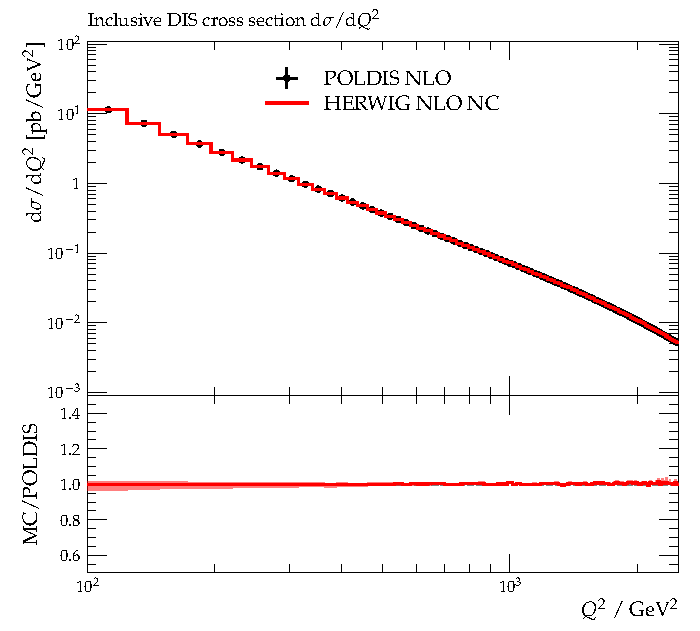
\includegraphics[width=0.32\linewidth]{figures/Q2PreCut.pdf}
  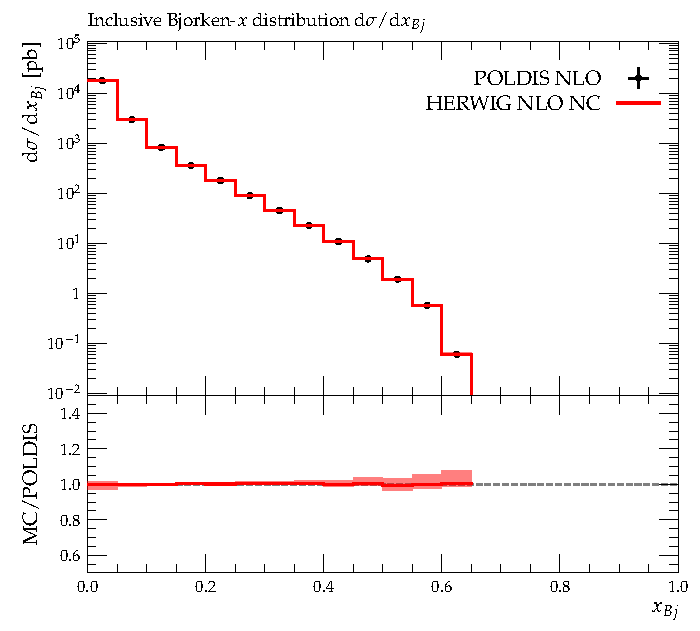
\includegraphics[width=0.32\linewidth]{figures/XBjPreCut.pdf}
  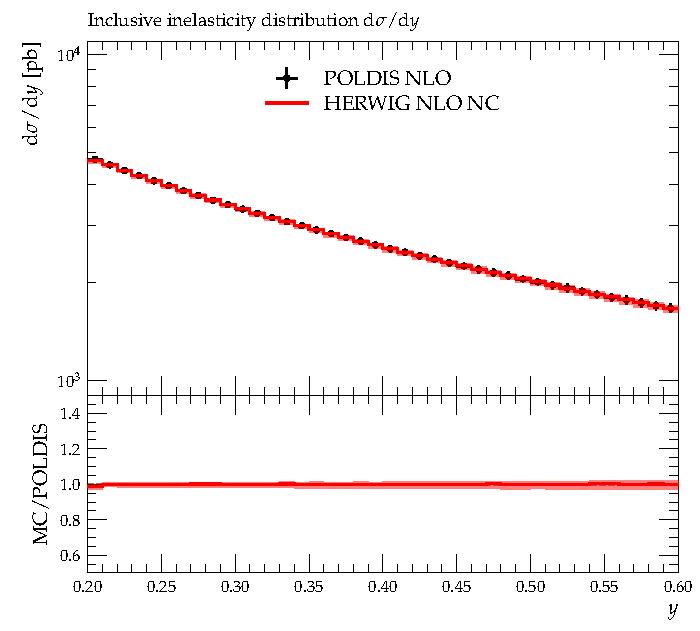
\includegraphics[width=0.32\linewidth]{figures/YPreCut.pdf}

  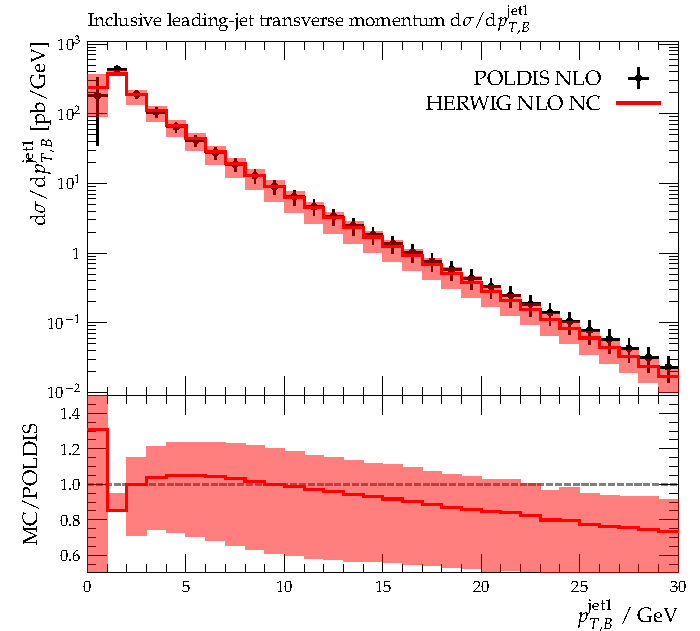
\includegraphics[width=0.32\linewidth]{figures/pT1PreCut.pdf}
  \includegraphics[width=0.32\linewidth]{figures/pT2PreCut.pdf}
  \caption{Inclusive unpolarized differential distributions before dijet cuts:
  $\mathrm{d}\sigma/\mathrm{d}Q^2$,
  $\mathrm{d}\sigma/\mathrm{d}x_{\mathrm{Bj}}$,
  $\mathrm{d}\sigma/\mathrm{d}y$,
  $\mathrm{d}\sigma/\mathrm{d}p_{T,1}^{B}$, and
  $\mathrm{d}\sigma/\mathrm{d}p_{T,2}^{B}$.}
  \label{fig:validation-diff-inclusive-unpol}
\end{figure}

\begin{figure}[!htbp]
  \centering
  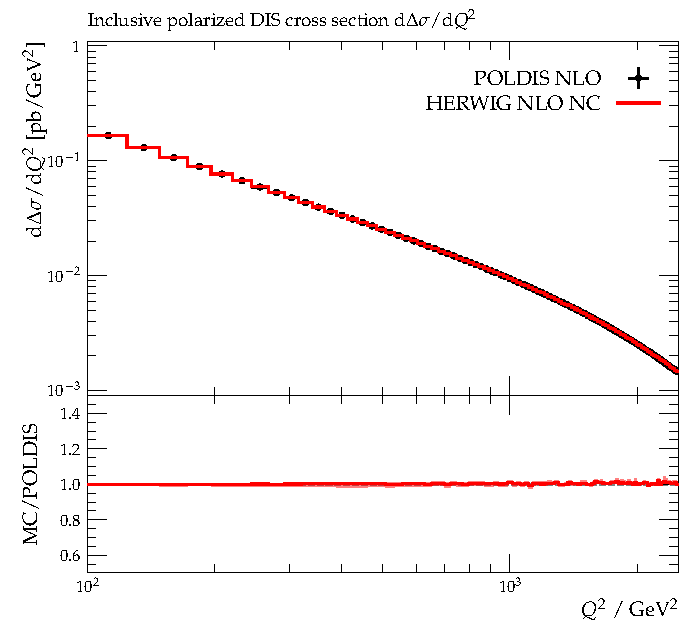
\includegraphics[width=0.32\linewidth]{figures/DQ2PreCut.pdf}
  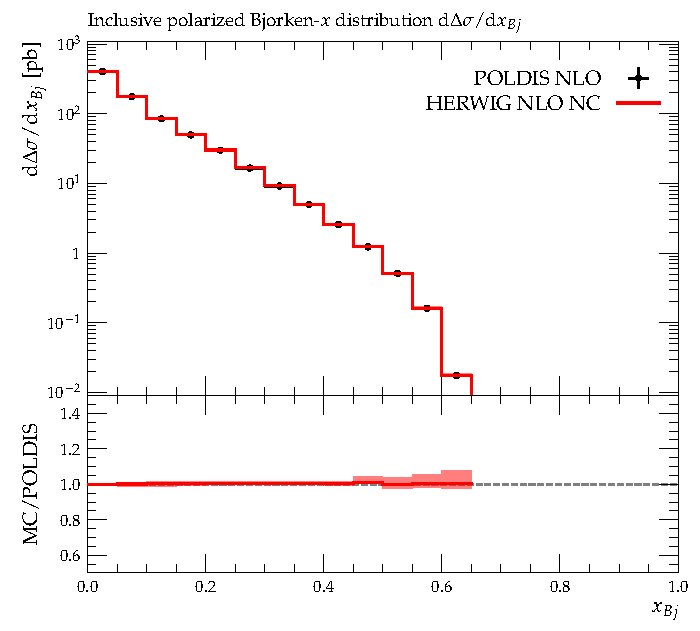
\includegraphics[width=0.32\linewidth]{figures/DXBjPreCut.pdf}
  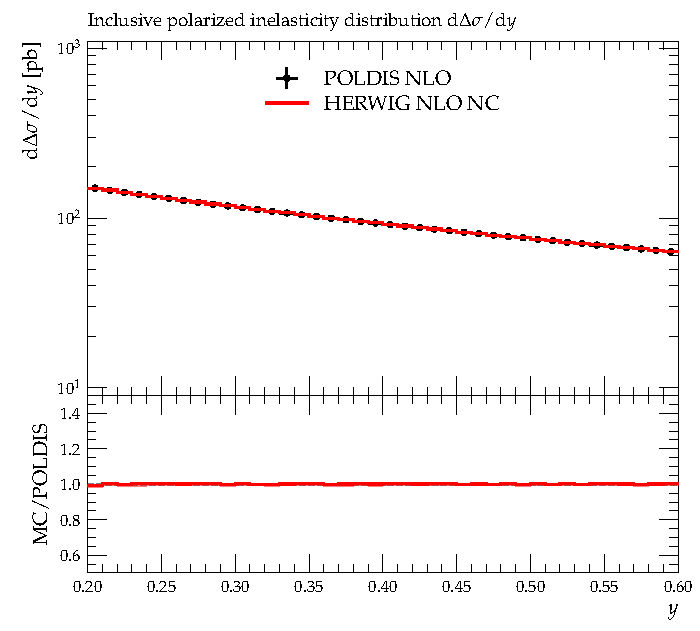
\includegraphics[width=0.32\linewidth]{figures/DYPreCut.pdf}

  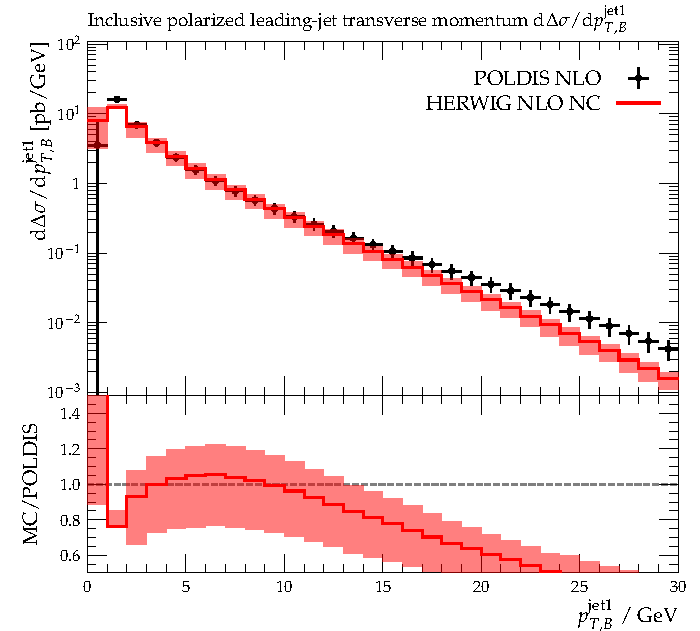
\includegraphics[width=0.32\linewidth]{figures/DpT1PreCut.pdf}
  \includegraphics[width=0.32\linewidth]{figures/DpT2PreCut.pdf}
  \caption{Inclusive polarized differential distributions before dijet cuts:
  $\mathrm{d}\Delta\sigma/\mathrm{d}Q^2$,
  $\mathrm{d}\Delta\sigma/\mathrm{d}x_{\mathrm{Bj}}$,
  $\mathrm{d}\Delta\sigma/\mathrm{d}y$,
  $\mathrm{d}\Delta\sigma/\mathrm{d}p_{T,1}^{B}$, and
  $\mathrm{d}\Delta\sigma/\mathrm{d}p_{T,2}^{B}$.}
  \label{fig:validation-diff-inclusive-pol}
\end{figure}

\begin{figure}[!htbp]
  \centering
  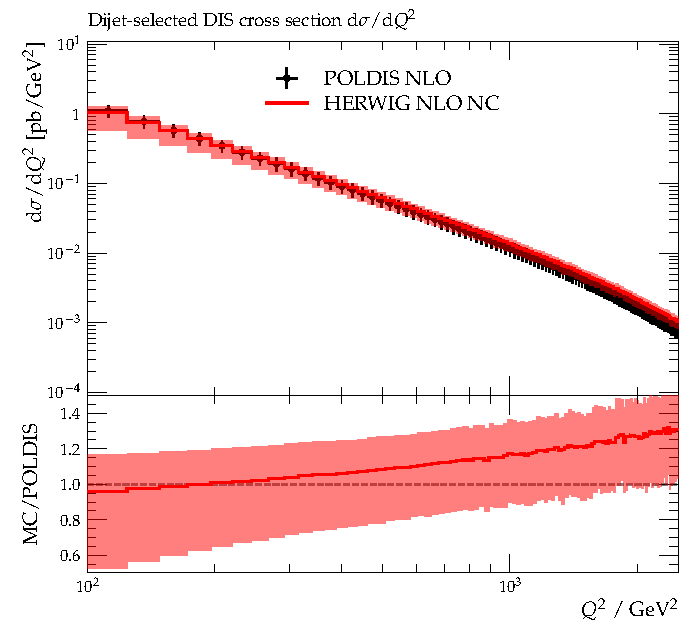
\includegraphics[width=0.32\linewidth]{figures/Q2.pdf}
  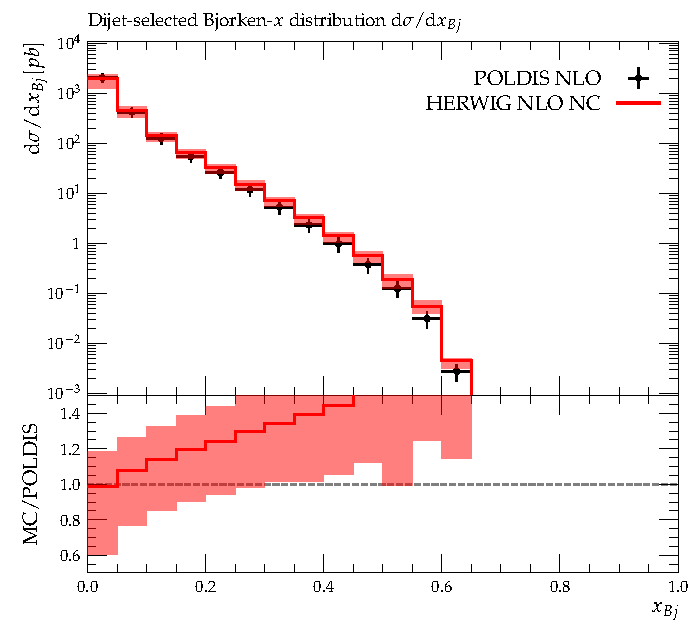
\includegraphics[width=0.32\linewidth]{figures/XBj.pdf}
  \includegraphics[width=0.32\linewidth]{figures/Pt.pdf}

  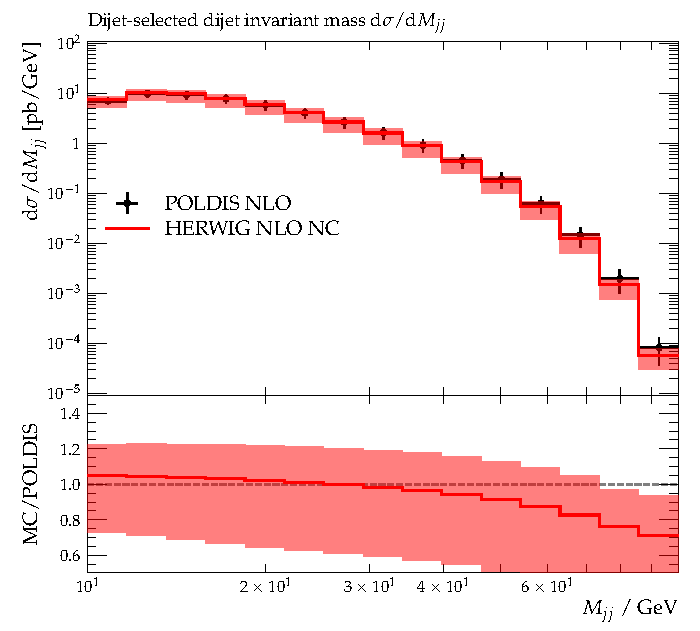
\includegraphics[width=0.32\linewidth]{figures/Mjj.pdf}
  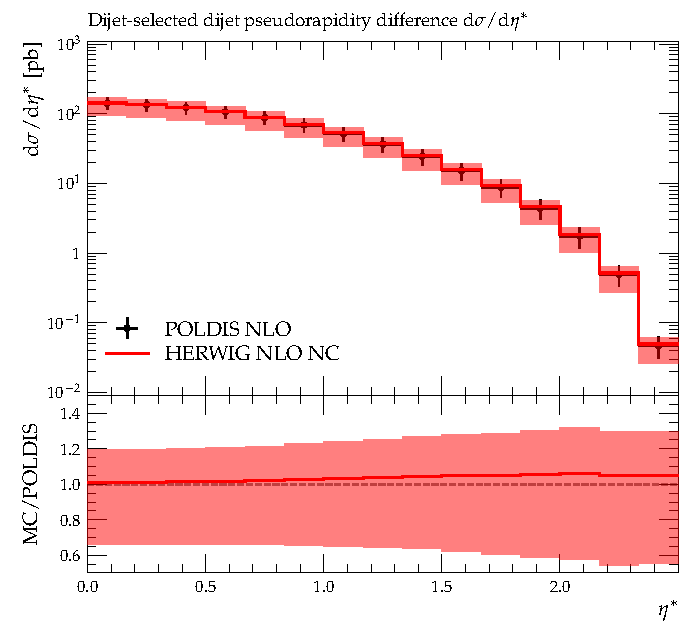
\includegraphics[width=0.32\linewidth]{figures/Eta.pdf}
  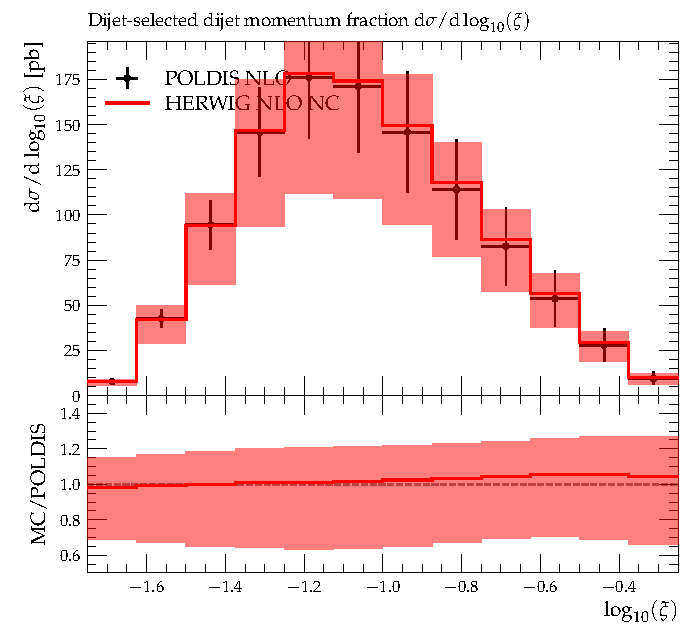
\includegraphics[width=0.32\linewidth]{figures/Zeta.pdf}
  \caption{Dijet-selected unpolarized kinematic distributions after dijet cuts:
  $\mathrm{d}\sigma/\mathrm{d}Q^2$,
  $\mathrm{d}\sigma/\mathrm{d}x_{\mathrm{Bj}}$,
  $\mathrm{d}\sigma/\mathrm{d}\langle p_T\rangle_2$,
  $\mathrm{d}\sigma/\mathrm{d}M_{jj}$,
  $\mathrm{d}\sigma/\mathrm{d}\eta^\ast$, and
  $\mathrm{d}\sigma/\mathrm{d}\log_{10}(\xi_2)$.}
  \label{fig:validation-diff-dijet-unpol-kin}
\end{figure}

\begin{figure}[!htbp]
  \centering
  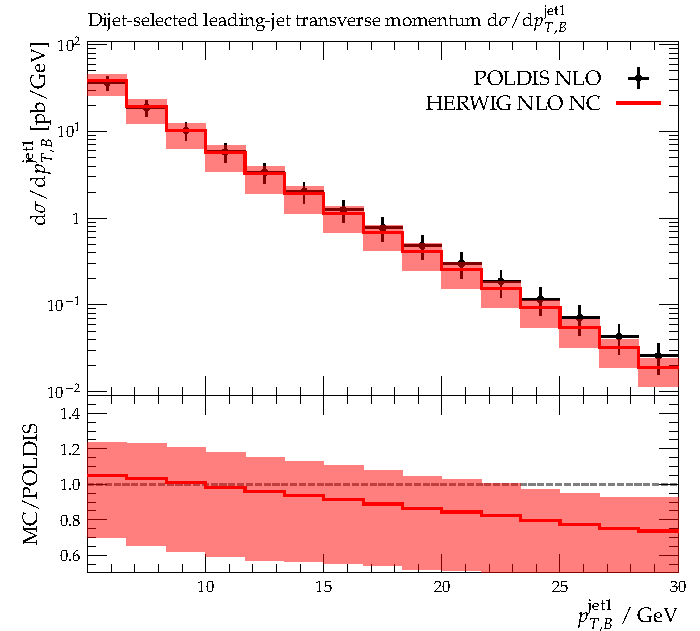
\includegraphics[width=0.47\linewidth]{figures/pT1.pdf}
  \includegraphics[width=0.47\linewidth]{figures/pT2.pdf}

  \includegraphics[width=0.47\linewidth]{figures/pT2OverpT1.pdf}
  \includegraphics[width=0.47\linewidth]{figures/pTAsym.pdf}
  \caption{Dijet-selected unpolarized jet-spectrum and balance distributions
  after dijet cuts:
  $\mathrm{d}\sigma/\mathrm{d}p_{T,1}^{B}$,
  $\mathrm{d}\sigma/\mathrm{d}p_{T,2}^{B}$,
  $\mathrm{d}\sigma/\mathrm{d}(p_{T,2}^{B}/p_{T,1}^{B})$, and
  $\mathrm{d}\sigma/\mathrm{d}A_{p_T}$.}
  \label{fig:validation-diff-dijet-unpol-balance}
\end{figure}

\begin{figure}[!htbp]
  \centering
  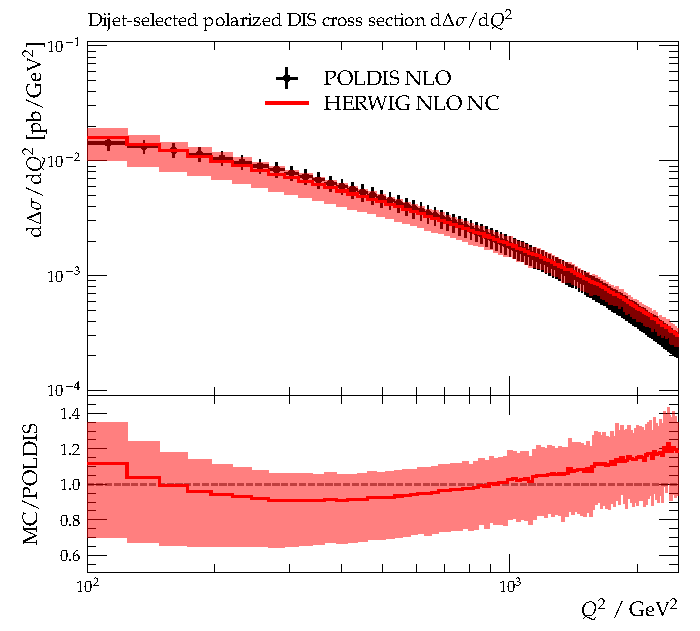
\includegraphics[width=0.32\linewidth]{figures/DQ2.pdf}
  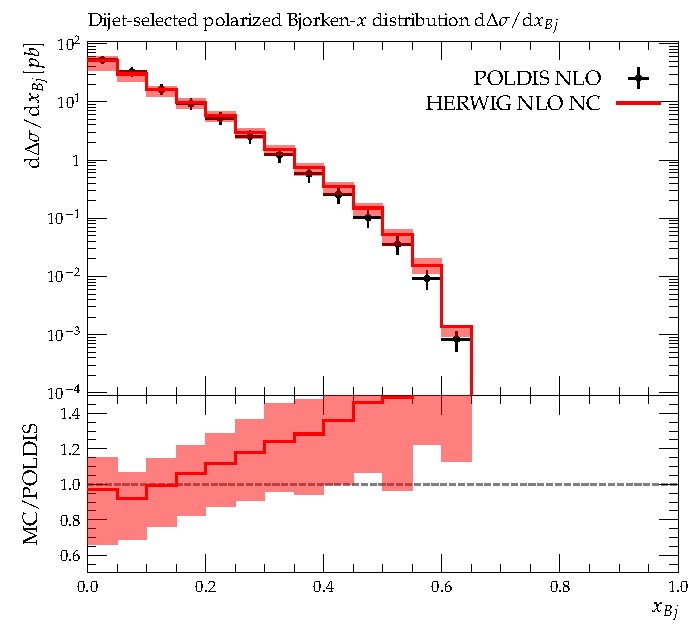
\includegraphics[width=0.32\linewidth]{figures/DXBj.pdf}
  \includegraphics[width=0.32\linewidth]{figures/DPt.pdf}

  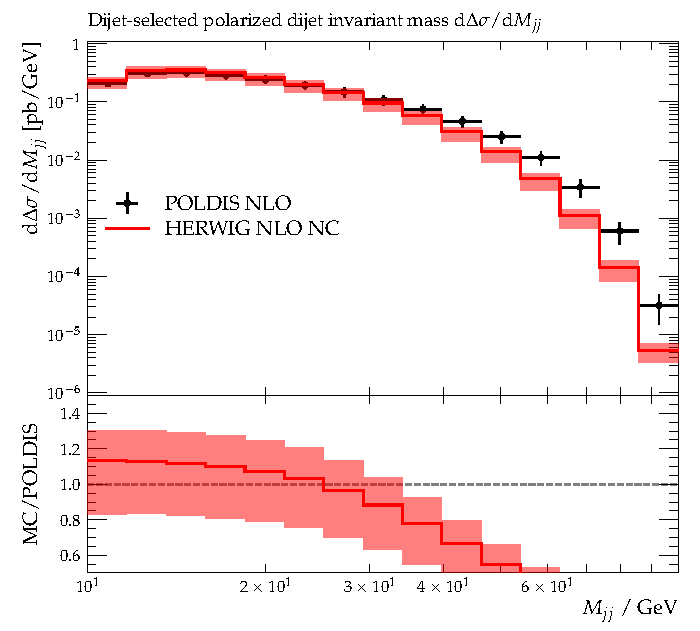
\includegraphics[width=0.32\linewidth]{figures/DMjj.pdf}
  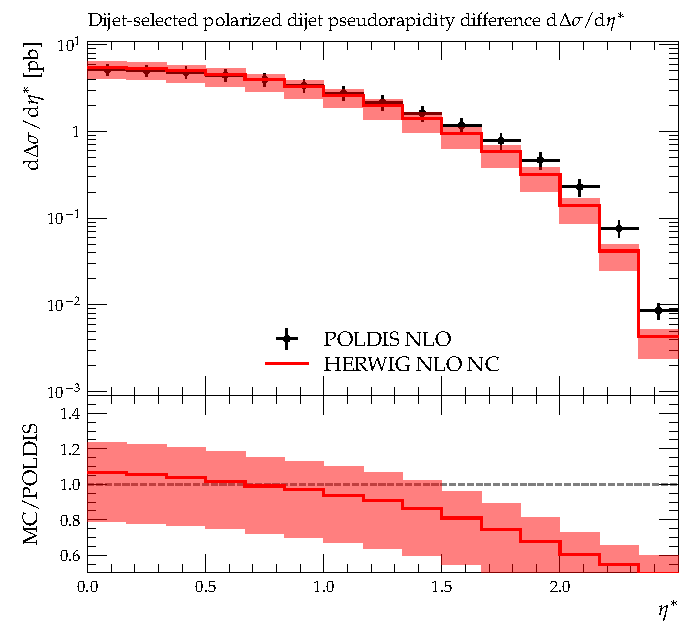
\includegraphics[width=0.32\linewidth]{figures/DEta.pdf}
  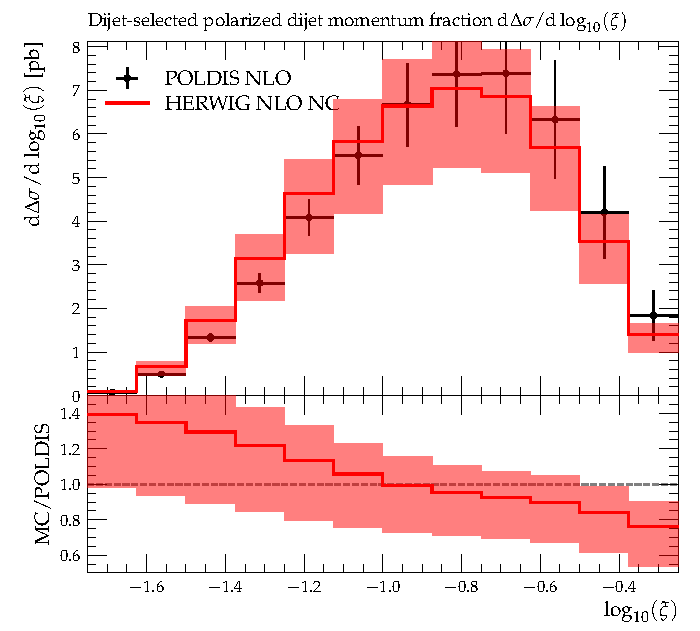
\includegraphics[width=0.32\linewidth]{figures/DZeta.pdf}
  \caption{Dijet-selected polarized kinematic distributions after dijet cuts:
  $\mathrm{d}\Delta\sigma/\mathrm{d}Q^2$,
  $\mathrm{d}\Delta\sigma/\mathrm{d}x_{\mathrm{Bj}}$,
  $\mathrm{d}\Delta\sigma/\mathrm{d}\langle p_T\rangle_2$,
  $\mathrm{d}\Delta\sigma/\mathrm{d}M_{jj}$,
  $\mathrm{d}\Delta\sigma/\mathrm{d}\eta^\ast$, and
  $\mathrm{d}\Delta\sigma/\mathrm{d}\log_{10}(\xi_2)$.}
  \label{fig:validation-diff-dijet-pol-kin}
\end{figure}

\begin{figure}[!htbp]
  \centering
  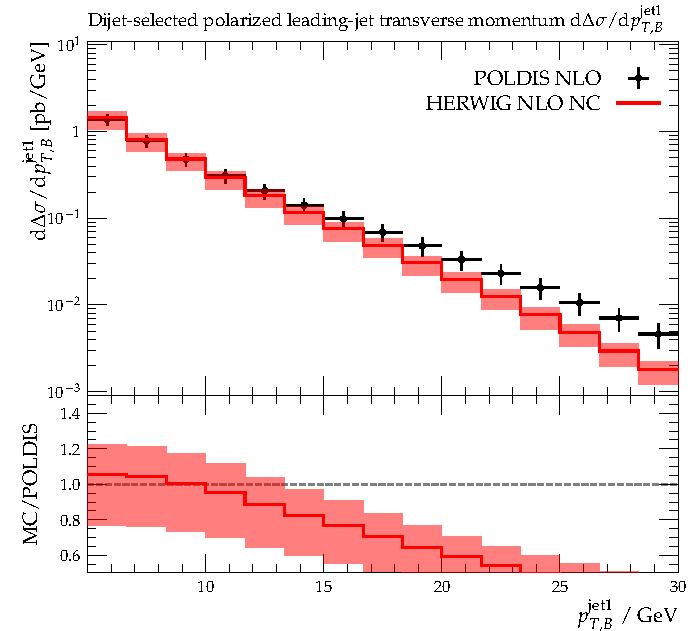
\includegraphics[width=0.47\linewidth]{figures/DpT1.pdf}
  \includegraphics[width=0.47\linewidth]{figures/DpT2.pdf}

  \includegraphics[width=0.47\linewidth]{figures/DpT2OverpT1.pdf}
  \includegraphics[width=0.47\linewidth]{figures/DpTAsym.pdf}
  \caption{Dijet-selected polarized jet-spectrum and balance distributions
  after dijet cuts:
  $\mathrm{d}\Delta\sigma/\mathrm{d}p_{T,1}^{B}$,
  $\mathrm{d}\Delta\sigma/\mathrm{d}p_{T,2}^{B}$,
  $\mathrm{d}\Delta\sigma/\mathrm{d}(p_{T,2}^{B}/p_{T,1}^{B})$, and
  $\mathrm{d}\Delta\sigma/\mathrm{d}A_{p_T}$.}
  \label{fig:validation-diff-dijet-pol-balance}
\end{figure}

\FloatBarrier
\subsection{Real-Emission Spin Information in the Shower}
\subsubsection{Details of the implementation}
In the standard \Herwig\ polarized-shower treatment, the spin
information of the incoming lepton and the Born-level hard process is propagated
through the subsequent branching history~\cite{Richardson:2018pvo}. At NLO,
however, the hardest POWHEG emission selects a realized $2\to 3$ partonic
configuration (i.e.\ the QCD Compton or boson--gluon fusion state) before the
shower begins, and this configuration carries additional spin information
beyond a purely Born-level description. To retain this information during
showering, the realized real-emission event is supplemented with an auxiliary
production vertex constructed from the exact helicity amplitudes for the
corresponding neutral-current DIS channels,
\begin{equation}
  e\,q \to e\,q\,g
  \qquad\text{and}\qquad
  e\,g \to e\,q\,\bar q\,.
\end{equation}
These amplitudes are evaluated with the same electroweak couplings and channel
assignments as in the validated polarized DIS matrix elements, so the spin
information attached to the event is consistent with the underlying neutral-current NLO
calculation. The charged-current implementation described earlier uses the same
hard-process framework, but the shower-spin study shown in this subsection is
restricted to the neutral-current case. In the current implementation, the accepted real-emission kernels reconstruct the incoming parton polarization at the mapped momentum fraction $x_B/x_p$; for neutral-current DIS this includes the exact mapped-even QCDC denominator factor and separate BGF $R_2/R_3$ analysing powers for the two charge-conjugate limits.

The role of this additional vertex is purely to supply the shower with the
appropriate spin-density information. The hardest-emission kinematics, flavour
channel, and colour flow remain those already selected by the POWHEG event
generation, and the accepted hard-event weights, the $\bar B$ function, and the
POWHEG hardest-emission selection are unchanged. The helicity amplitudes are
used solely to construct the spin-density matrix of the outgoing particles;
neither the event weight nor the emission probability is altered. This
means that the spin-dependent shower evolution modifies only subleading
post-hardest-emission correlations and does not alter the NLO accuracy of the
matched hard cross section. This
separation allows the impact of the additional real-emission spin information
to be studied in shower-sensitive observables without obscuring the fixed-order
validation of the hard process.

Operationally, the incoming lepton density matrix is inherited from the DIS
state, while the incoming parton polarization is reconstructed from the beam
polarization and the polarized PDFs at the momentum fraction associated with
the realized emission. The resulting spin vertex then defines the density
matrices carried by the outgoing lepton and by the two outgoing coloured legs.
This extends the shower initialization procedure described in
Section~\ref{sec:formalism}. In the standard algorithm, spin correlations are
initialized from the Born-level density matrix; here that object is replaced by
the density matrix of the full real-emission state.
For completeness, a short description of the one-remnant fallback used in some
DIS event-generation configurations is collected in Appendix~\ref{app:dis-remnant-fallback}.

\subsubsection{Validation of the Spin Correlations}
The fixed-order comparisons discussed above validate the polarized DIS matrix
elements and their combination into inclusive and dijet-selected cross sections. A
separate NLO+PS validation is needed to isolate the effect of propagating the
spin information from the exact real-emission configuration into the polarized
shower. For this purpose we use the same post-dijet event sample as in the
Breit-frame dijet analysis: the event must satisfy the DIS window
$49 \le Q^2 \le 2500~\mathrm{GeV}^2$ and $0.2 \le y \le 0.6$, and the two
leading Breit-frame jets must pass
$p_{T,1}^{B}>5~\mathrm{GeV}$,
$p_{T,2}^{B}>4~\mathrm{GeV}$, and
$-3.5<y_{\mathrm{lab}}<3.5$.

The spin-correlation validation then compares three shower configurations:
\begin{itemize}
\item \textbf{Full}: the POWHEG real-spin vertex is enabled and the shower spin
  correlations are enabled;
\item \textbf{Born-Only}: the POWHEG real-spin vertex is disabled while the
  shower spin correlations remain enabled;
\item \textbf{None}: both the POWHEG real-spin vertex and the shower spin
  correlations are disabled.
\end{itemize}
This separation allows one to disentangle the new real-emission
spin information from the spin dependence already present in the Born-level
DIS configuration.

The particle-level observables are constructed from visible stable particles in
the Breit-frame current hemisphere, excluding the scattered lepton. If
$s_{\mathrm{DIS}}=\pm1$ denotes the DIS orientation sign returned by the
Breit-frame kinematics convention, the current hemisphere is defined by
\begin{equation}
  s_{\mathrm{DIS}}\,p_{z,i}^{B}<0\,.
\end{equation}
This follows the standard Breit-frame current-hemisphere construction used in
DIS event-shape studies~\cite{Dasgupta:2003iq,Gehrmann:2019hwf,H1:2006eventshapes,ZEUS:2007eventshapes}. The corresponding
current-hemisphere broadening is
\begin{equation}
  B_C
  \equiv
  \frac{\sum_{i\in \mathrm{CH}} p_{T,i}^{B}}
       {2\sum_{i\in \mathrm{CH}} |\vec{p}_i^{\,B}|}\,,
\end{equation}
which is the standard current-hemisphere, or boson-axis, broadening used in
Breit-frame DIS event-shape analyses~\cite{Dasgupta:2003iq,Gehrmann:2019hwf,H1:2006eventshapes,ZEUS:2007eventshapes}.

For the ordinary differential observables we construct the double-spin
asymmetry
\begin{equation}
  A_{LL}(O)=\frac{\Delta\sigma(O)}{\sigma(O)}\,,
\end{equation}
where, in the analysis presented here,
\begin{equation}
  \Delta\sigma(O)=\sigma^{++}(O)-\sigma^{+-}(O)-\sigma^{-+}(O)+\sigma^{--}(O)\;,
\end{equation}
with the first superscript referring to the lepton helicity and the second to the hadron helicity, while $\sigma(O)$ is the sum of the same four helicity configurations. Relative to the integrated observables defined earlier, the common factor of $1/4$ is omitted here because it cancels identically in the ratio $A_{LL}$. This construction is used for observables such as
$p_{T,3}^{B}$ and $p_{T,3}^{B}/p_{T,1}^{B}$.

Observables controlled
primarily by the hard process should continue to provide closure tests and
remain stable across the three configurations. The strongest differences are
instead expected in radiation-sensitive observables, in particular
$p_{T,3}^{B}$, $p_{T,3}^{B}/p_{T,1}^{B}$, and the cumulative broadening
asymmetry defined below. Within this setup
the cleanest discriminator of the new real-emission spin information is the
comparison of \textbf{Full} to \textbf{Born-Only}, while \textbf{None}
provides the baseline with no shower spin correlations.

The resulting phenomenology is naturally organized into two classes of
observables. The first is represented by the third-jet distributions collected
in Fig.~\ref{fig:spincomp-pt3}. The Breit-frame third-jet transverse momentum
and the ratio $p_{T,3}^{B}/p_{T,1}^{B}$ are directly sensitive to additional
resolved radiation beyond the leading dijet system, and therefore provide a
clean test of how much spin information survives into the extra-radiation
pattern. The comparison of \textbf{Full}, \textbf{Born-Only}, and \textbf{None}
is intended to separate the effect of the real-emission spin vertex from the
baseline shower spin correlations.

\begin{figure}[!htbp]
  \centering
  \safegraphic{0.47\linewidth}{figures/pT3.pdf}
  \hfill
  \safegraphic{0.47\linewidth}{figures/pT3OverpT1.pdf}
  \caption{Third-jet observables in the spin-comparison study. Left: the
  Breit-frame third-jet transverse-momentum distribution
  $\mathrm{d}\sigma/\mathrm{d}p_{T,3}^{B}$. Right:
  $\mathrm{d}\sigma/\mathrm{d}(p_{T,3}^{B}/p_{T,1}^{B})$. These observables
  are used to test how the \textbf{Full}, \textbf{Born-Only}, and \textbf{None}
  shower configurations modify the pattern of additional radiation beyond the
  leading dijet system.}
  \label{fig:spincomp-pt3}
\end{figure}

The second class is represented by the cumulative current-hemisphere
broadening asymmetry shown in Fig.~\ref{fig:spincomp-broadening}. This provides
the most direct handle on the additional spin information carried by the
realized NLO emission. Since the underlying broadening variable $B_C$ receives
contributions from all particles in the current hemisphere, it is sensitive to
multiple wide-angle emissions and their recoil, and is therefore the natural
place to look for accumulated spin-dependent changes in the radiation pattern.
The comparison of \textbf{Full} and \textbf{Born-Only} tests whether the
realized-emission spin vertex induces an effect beyond the shower correlations
already generated from the polarized Born-level configuration.

To stabilize the statistically sparse high-$B_C$ region, we focus on the
cumulative quantity
\begin{equation}
  A_{LL}(B_C > B_C^{\mathrm{cut}})
  \equiv
  \frac{\Delta\sigma(B_C > B_C^{\mathrm{cut}})}
       {\sigma(B_C > B_C^{\mathrm{cut}})}\,,
\end{equation}
which integrates the broadening tail from above and provides a robust summary
of the same trend.

\begin{figure}[!htbp]
  \centering
  \safegraphic{0.62\linewidth}{figures/ALLBroadeningCumulative.pdf}
  \caption{Cumulative broadening asymmetry used to isolate the effect of the
  real-emission spin vertex:
  $A_{LL}(B_C > B_C^{\mathrm{cut}})$. This observable integrates the
  current-hemisphere broadening tail from above. The comparison of
  \textbf{Full} and \textbf{Born-Only} provides the most direct test of the
  additional spin information associated with the realized NLO emission, while
  \textbf{None} supplies the no-spin baseline.}
  \label{fig:spincomp-broadening}
\end{figure}

\FloatBarrier
\subsubsection{Impact of Hadronization}
To assess the extent to which the shower-level effects discussed above persist
after non-perturbative evolution, we also compare predictions obtained with
hadronization disabled and enabled. In order to keep the presentation compact,
the main text restricts this comparison to the \textbf{Full} configuration and
to two representative observables: the third-jet transverse momentum
$p_{T,3}^{B}$ and the cumulative broadening asymmetry
$A_{LL}(B_C > B_C^{\mathrm{cut}})$. The first probes the stability of the
additional-radiation pattern under hadronization, while the second provides a
compact summary of the broadening tail. The corresponding comparison is shown
in Fig.~\ref{fig:hadronization-main}. Additional supporting comparisons are
deferred to Appendix~\ref{app:hadronization-extra}.

\begin{figure}[!htbp]
  \centering
  \safegraphic{0.47\linewidth}{figures/pT3Hadronization.pdf}
  \hfill
  \safegraphic{0.47\linewidth}{figures/ALLBroadeningCumulativeHadronization.pdf}
  \caption{Hadronization study in the \textbf{Full}
  configuration. Left: comparison of the third-jet transverse-momentum
  distribution with hadronization disabled and enabled. Right: comparison of
  the cumulative broadening asymmetry
  $A_{LL}(B_C > B_C^{\mathrm{cut}})$ in the same two setups.}
  \label{fig:hadronization-main}
\end{figure}

\FloatBarrier
\section{Summary and Outlook}\label{sec:conclusions}

We have presented the implementation of polarized deep-inelastic scattering at next-to-leading order in \Herwig\ using the POWHEG matching scheme. The implementation covers the full neutral-current process, including $\gamma/Z$ interference, as well as the charged-current channel. The real-emission contributions for both the QCD Compton and boson--gluon fusion channels have been derived, together with the virtual corrections and collinear counterterms needed for NLO event generation. Integrated cross sections have been compared with the fixed-order program \POLDIS, with agreement at the permille level for the dominant channels and at the percent level for the smaller polarized interference contributions. The differential hardest-emission proxy comparisons give agreement ranging from a few percent to $\mathcal{O}(10\%)$, depending on the observable and its sensitivity to the POWHEG Sudakov treatment and the dijet acceptance.

A second key result is the consistent propagation of spin correlations from the NLO real-emission state to the parton shower. By initializing the shower with the exact spin-density matrix of the accepted real-emission configuration, the full spin information of the POWHEG event is retained without modifying the accepted hard-event normalization or POWHEG emission choice. We have introduced a set of third-jet observables together with the cumulative current-hemisphere broadening asymmetry that provide an exploratory probe of the impact of this additional spin information in showered events.

Several extensions suggest themselves. It will be important to systematize the
comparison across a broader set of jet- and particle-level observables. A
quantitative study of the stability of the resulting effects under variations
of shower and hadronization settings is likewise needed. More broadly, the
formalism developed here provides the necessary ingredients for treating
polarized hard scattering in \Herwig\ beyond DIS, thereby opening the way to
polarized processes at hadron--hadron and lepton--hadron colliders.

\section*{Acknowledgments}
We would like to thank Daniel de Florian for useful discussions and for providing the \POLDIS\ code used for validation. AP acknowledges support from the US Department of Energy, Office of Science, Office of Nuclear Physics under Award Number DE-SC0025728.
\appendix

\section{DIS One-Remnant Fallback}
\label{app:dis-remnant-fallback}

For DIS configurations with only one beam remnant, we introduce a small extension
to the \Herwig\ remnant handler in the form of the
\texttt{DISOneRemnantFallback} option. Only two settings are retained:
\texttt{Default} and \texttt{RelaxMass}.

The default behaviour leaves the standard \Herwig\ remnant treatment unchanged:
if the selected recoil system cannot support an on-shell remnant with the
nominal remnant mass, the event is vetoed. The \texttt{RelaxMass} option keeps
the same recoil construction, but if that final on-shell projection fails it
reduces the effective one-remnant mass to the largest kinematically allowed
value and proceeds with that reshuffle instead of vetoing the event. In other
words, the option does not change the hard-process selection or the recoil
system; it only modifies the final one-remnant mass constraint when that
constraint would otherwise abort the event.

In plain terms, \texttt{RelaxMass} is therefore a last-resort kinematic repair:
the event keeps the same hard process and the same recoil assignment, but the
single remnant is made lighter if that is the only way to put it on shell after
the reshuffle. We did not monitor the trigger frequency of this fallback in the
production runs used for the present study, so we do not make a quantitative
statement here about how often it is invoked in practice.

This fallback does not alter the underlying hard process or introduce a new recoil scheme;
it simply replaces an otherwise fatal on-shell remnant failure by the closest
kinematically allowed one-remnant configuration.

\section{Additional Hadronization Comparisons}
\label{app:hadronization-extra}

This appendix provides a more targeted comparison designed to test
whether hadronization modifies the separation between the spin-correlation
treatments themselves. For this purpose we consider only the cumulative
broadening asymmetry $A_{LL}(B_C > B_C^{\mathrm{cut}})$ at hadron level, shown
for the \textbf{Full}, \textbf{Born-Only}, and \textbf{None} configurations on
the same graph. This keeps the supporting material focused on the observable
that is most directly sensitive to the residual \textbf{Full} versus
\textbf{Born-Only} effect, while avoiding an unnecessary proliferation of
appendix figures.

\begin{figure}[!htbp]
  \centering
  \safegraphic{0.62\linewidth}{figures/ALLBroadeningCumulativeHadronLevelComparison.pdf}
  \caption{Comparison of
  $A_{LL}(B_C > B_C^{\mathrm{cut}})$ showing the
  \textbf{Full}, \textbf{Born-Only}, and \textbf{None} predictions after
  hadronization on the same graph, in order to assess whether hadronization
  changes the separation between the spin treatments.}
  \label{fig:hadronization-appendix}
\end{figure}

\clearpage
% Bibliography
\bibliographystyle{JHEP}
\bibliography{biblio}

\end{document}
